\documentclass[11pt,magyar,a4paper,twoside,]{report}
\usepackage[T1]{fontenc}
\usepackage{ae}
\usepackage{lmodern}
\usepackage{amssymb}
\usepackage{amsmath}
\usepackage{ifxetex,ifluatex}
\usepackage{fixltx2e} % provides \textsubscript
\usepackage{adjustbox}
\usepackage[thmmarks]{ntheorem}
\usepackage{listings}
\usepackage{color}
\usepackage{lastpage}
\usepackage{anysize}
\usepackage{longtable}
\usepackage{sectsty}
\usepackage{setspace}
\usepackage[hang]{caption}
\usepackage{tabularx}
\usepackage{hyphenat}
\usepackage{enumitem}
\usepackage{subcaption}
\usepackage{todonotes}
\usepackage{adjustbox}
\usepackage{minibox}
\usepackage{pdfpages}
\usepackage{tikz}
\usepackage{float}
% fix for pandoc 1.14
\providecommand{\tightlist}{%
  \setlength{\itemsep}{0pt}\setlength{\parskip}{0pt}}
% use microtype if available
\IfFileExists{microtype.sty}{\usepackage{microtype}}{}
% use upquote if available, for straight quotes in verbatim environments
\IfFileExists{upquote.sty}{\usepackage{upquote}}{}
\ifnum 0\ifxetex 1\fi\ifluatex 1\fi=0 % if pdftex
  \usepackage[utf8]{inputenc}
\else % if luatex or xelatex
  \usepackage{fontspec}
  \ifxetex
    \usepackage{xltxtra,xunicode}
  \fi
  \defaultfontfeatures{Mapping=tex-text,Scale=MatchLowercase}
  \newcommand{\euro}{€}
\fi
\usepackage{natbib}
\bibliographystyle{plain}
\usepackage{graphicx}
% We will generate all images so they have a width \maxwidth. This means
% that they will get their normal width if they fit onto the page, but
% are scaled down if they would overflow the margins.
\makeatletter
\def\maxwidth{\ifdim\Gin@nat@width>\linewidth\linewidth
\else\Gin@nat@width\fi}
\makeatother
\let\Oldincludegraphics\includegraphics
%\renewcommand{\includegraphics}[1]{\Oldincludegraphics[scale=1.0]{#1}}
\renewcommand{\includegraphics}[1]{
\begin{adjustbox}{max size={\textwidth}{\textheight}}
    \Oldincludegraphics[scale=0.6]{#1}%
\end{adjustbox}
}
\ifxetex
  \usepackage[setpagesize=false, % page size defined by xetex
              unicode=false, % unicode breaks when used with xetex
              xetex]{hyperref}
\else
  \usepackage[unicode=true]{hyperref}
\fi
\definecolor{darkgreen}{rgb}{0,0.5,0}
\hypersetup{breaklinks=true,
            bookmarks=true,
            pdfauthor={},
            pdftitle={},
            colorlinks=true,
            urlcolor=blue,
            linkcolor=magenta,
            citecolor=darkgreen,
            pdfborder={0 0 0}}
\urlstyle{same}  % don't use monospace font for urls
\setlength{\parindent}{0pt}
\setlength{\parskip}{6pt plus 2pt minus 1pt}
\setlength{\emergencystretch}{3em}  % prevent overfull lines
\ifxetex
  \usepackage{polyglossia}
  \setmainlanguage{}
\else
  \usepackage[magyar]{babel}
\fi

\title{Mikroszolgáltatásokra épülő architektúra fejlesztésének és tesztelésének támogatása}
\author{Borlay Dániel}

\renewcommand*{\hyperref}[2][\ar]{%
  \def\ar{#2}
  #2 (\refstruc{#1})}

\renewcommand*{\figureautorefname}{ábra}

\sloppy

% for English documents
%\setlength{\parindent}{0pt} % áttekinthetőbb, angol nyelvű dokumentumokban jellemző
%\setlength{\parskip}{8pt plus 3pt minus 3pt} % áttekinthetőbb, angol nyelvű dokumentumokban jellemző

% for Hungarian documents
\setlength{\parindent}{12pt}
\setlength{\parskip}{0pt}

\marginsize{35mm}{25mm}{15mm}{15mm} % anysize package
\setcounter{secnumdepth}{0}
\sectionfont{\large\upshape\bfseries}
\setcounter{secnumdepth}{3}
\singlespacing
\frenchspacing


\begin{document}

\footnotesize


\normalsize

%--------------------------------------------------------------------------------------
% The title page
%--------------------------------------------------------------------------------------
\begin{titlepage}
\begin{center}
\Oldincludegraphics[width=60mm,keepaspectratio]{img/BME1782logo.pdf}\\

\vspace{0.3cm}
\textbf{Budapesti Műszaki és Gazdaságtudományi Egyetem}\\
\textmd{Méréstechnika és Információs Rendszerek Tanszék}\\
\textmd{}\\[5cm]

\vspace{0.4cm}
{\huge \bfseries Mikroszolgáltatásokra épülő architektúra fejlesztésének és tesztelésének támogatása}\\[0.8cm]
\vspace{0.5cm}
\textsc{\Large Diplomaterv}\\[4cm]

\begin{tabular}{cc}
 \makebox[7cm]{\emph{Készítette}} & \makebox[7cm]{\emph{Konzulens}} \\
 \makebox[7cm]{Borlay Dániel} & \makebox[7cm]{Szatmári Zoltán}
\end{tabular}

\vfill
{\large \today}
\end{center}
\end{titlepage}

\onehalfspacing

\hypersetup{linkcolor=black}
\setcounter{tocdepth}{2}
\tableofcontents

\vfill
\clearpage

\begin{center}
\large
\textbf{HALLGATÓI NYILATKOZAT}\\
\end{center}

Alulírott \emph{Borlay Dániel}, szigorló hallgató kijelentem, hogy ezt a diplomatervet meg nem engedett segítség nélkül, saját magam készítettem, csak a megadott forrásokat (szakirodalom, eszközök stb.) használtam fel. Minden olyan részt, melyet szó szerint, vagy azonos értelemben, de átfogalmazva más forrásból átvettem, egyértelműen, a forrás megadásával megjelöltem.

Hozzájárulok, hogy a jelen munkám alapadatait (szerző(k), cím, angol és magyar nyelvű tartalmi kivonat, készítés éve, konzulens(ek) neve) a BME VIK nyilvánosan hozzáférhető elektronikus formában, a munka teljes szövegét pedig az egyetem belső hálózatán keresztül (vagy autentikált felhasználók számára) közzétegye. Kijelentem, hogy a benyújtott munka és annak elektronikus verziója megegyezik. Dékáni engedéllyel titkosított diplomatervek esetén a dolgozat szövege csak 3 év eltelte után válik hozzáférhetővé.

\begin{flushleft}
\vspace*{1cm}
Budapest, \today
\end{flushleft}

\begin{flushright}
 \vspace*{1cm}
 \makebox[7cm]{\rule{6cm}{.4pt}}\\
 \makebox[7cm]{\emph{Borlay Dániel}}\\
 \makebox[7cm]{hallgató}
\end{flushright}
\thispagestyle{empty}

\vfill
\clearpage
\thispagestyle{empty} % an empty page

\chapter*{Kivonat}\label{kivonat}
\addcontentsline{toc}{chapter}{Kivonat}

Napjainkban komoly gondot okoz, hogy hogyan lehet hatékonyan elosztott,
jó rendelkezésre állású, könnyen skálázható alkalmazást építeni. Sok
architektúrális megközelítés van, amit alapul véve hatákonyan
tervezhetjük meg a rendszerünket, és könnyen elkészíthetjük az
alkalmazásunkat. Egy ilyen architektúrális megközelítés a
mikroszolgáltatásokon alapuló architektúra, amivel apró részletekre
bontva a feladatot, könnyen kezünkben tarthatjuk az elosztott
alkalmazásunkat.

A diplomaterv keretében az volt a feladatom, hogy megismerjem az
architektúra lényegét és müködését, illetve kiderítsem, hogy milyen
eszközökkel tudom automatizálás segítségével támogatni a fejlesztés, és
működtetés folyamatát.

A diplomaterv célkitűzése, hogy egy olyan mikroszolgáltatásokra épülő
alkalmazást készítsek, amellyel be tudom mutatni az architektúra
előnyeit, végig tudom vezetni rajta a tesztelés folyamatát, tudom
automatizálni a tesztelését, és működtetését, és betekintést tudok adni
az architektúrához használatos technológiákba.

\chapter*{Abstract}\label{abstract}
\addcontentsline{toc}{chapter}{Abstract}

Nowadays it's a very big problem, that how to build a distributed,
highly available, easily scalable application efficiently. There are
many ways to design our system and application which we could base on
our plans. One of these design patterns is the microservice based
architecture, which creates small services from the big application, by
separating the functionality, and we can handle more efficiently our
distributed application.

The goal of this thesis is to gather knowledge about the architecture,
how it works or how it could be designed, or which continuous
integration tool could be used for helping development and maintenance.

The goal of this thesis is to create and example application based on
microservice architecture, which could be used for showing the
advantages of the technique, and I can show the full process of testing
and I can create a framework for helping the development of the
application by automated testing and integration.

\chapter{Bevezetés}\label{bevezetuxe9s}

Fontos, hogy az alkalmazásaink megbízhatóan, karbantarthatóan, és nagy
rendelkezésre állással legyenek elérhetőek. Napjaink egyik feltörekvő
architektúra építési elve a mikroszolgáltatások archtektúrája. Ezt az
architektúra típust az elosztott működése, a szolgáltatásonkénti könnyen
fejleszthetősége, és a jó skálázhatósága teszi népszerűvé. Sok cég
választja ezt az új elvet, mivel az egyes komponensek fejlesztése
egyszerűbb és gyorsabb, a végeredmény pedig könnyebben karbantartható,
és egyszerűen számítási felhőbe integrálható.

Jelen labor keretében megismerkedem a mikroszolgáltatások felépítésével,
működésével, és egy automatizált megoldást adok a használatukra.
Bemutatom, hogy hogyan lehet azt a technológiát automatizáltan
tesztelni, és a fejlesztési folyamatot egyszerűen és felügyelve vezetni.

Az második fejezetben beleástam magam a technológiai áttekintésbe, ahol
az architektúra lényegét próbáltam megérteni, és összeszedtem, hogy
milyen tervezési kérdések merülnek fel egy mikroszolgáltatásokra épülő
alkalmazás elkészítésénél.

A harmadik fejezetben megnéztem, hogy milyen előnyei illetve hátrányai
lehetnek ennek a módszernek, illetve megnéztem egy példát
(Archivematica), ami segíthet az átfogó kép alkotásában, és saját
alkalmazás fejlesztésében.

A negyedik fejezetben a kapcsolódó technológiákról készítettem egy
összefoglalást, ami tartalmazza a jelenleg használt technológiákat,
amikkel mikroszolgáltatásokra épülő architektúrát lehet építeni, illetve
olyan technológiákat, amikkel kiegészítve teljesen felügyelhető a
szolgáltatások működése.

Az ötödik fejezetben a különböző kommunikációs lehetőségekkel
foglalkoztam, amikkel össze lehet kötni a szolgáltatásokat, illetve a
kommunikáció tervezése közben felmerülő nehézségeket néztem át.

A hatodik fejezetben megterveztem a példa alkalmazást, illetve az
architektúrát, amit meg fogok alkotni a diplomaterv során.

A hetedik fejezetben az alkalmazás implementációját járom körbe.

A nyolcadik fejezetben az elkészítés közben tapasztalt nehézségeket, és
az alkalmazás értékelését fejtem ki bővebben.

A kilencedik fejezetben az automatizálást járom körbe, kitérek arra,
hogy mit hogyan célszerű csinálni egy mikroszolgáltatásokra épülő
automatizált rendszerben, és mit lehet véghez vinni az általam
elkészített struktúrában.

A tizedik fejezetben a valós felhasználási módokat mutatom be, és
kifejtem, hogy mikor és milyen körülmények között van értelme az
automatizált támogatásnak és a mikroszolgáltatások használatának.

A tizenegyedik fejezet tartalmazza az összefoglalást, ami egy értékelést
ad az elvégzett munkáról. Ebben a fejezetben térek ki a diploma munka
lehetséges folytatási lehetőségeire.

\chapter{Háttérismeretek}\label{huxe1ttuxe9rismeretek}

\section{Mikroszolgáltatások}\label{mikroszolguxe1ltatuxe1sok}

A mikroszolgáltatás\citep{microservices} \citep{micro-arch}
\citep{microservices-light} egy olyan architektúrális modellezési mód,
amikor a tervezett rendszert/alkalmazást kisebb funkciókra bontjuk, és
önálló szolgáltatásokként, önálló erőforrásokkal, valamilyen jól
definiált interfészen keresztül tesszük elérhetővé.

Ezt az architektúrális mintát az teszi erőssé, hogy nem függenek
egymástól a különálló komponensek, és csak egy kommunikációs interfészt
ismerve is karbantartható a rendszer. Egy szoftver fejlesztési
projektben előnyös lehet, hogy az egyes csapatok fókuszálhatnak a saját
szolgáltatásukra, és nincs szükség a folyamatos kompatibilitás
tesztelésére.

Egy mikroszolgáltatást használó architektúra kiépítéséhez sokféle
funkcionális elkülönítési módot használnak, amivel a szolgáltatásokat
kialakíthatjuk. Egy ilyen elválasztásí módszer a rendszer
specifikációjában lévő főnevek vagy igék kiválasztása, és az így kapot
halmaz felbontása. Egy felbontás akkor minősül ideálisnak, ha nem tudjuk
tovább bontani az adott funkciót. A valóságban soha nem lesz az
ideálisnak megfelelő felbontás, mivel erőforrás pazalró, és túlzottan
elosztott rendszert kapnánk.

\subsection{Szolgáltatás elválasztás
tervezése}\label{szolguxe1ltatuxe1s-elvuxe1lasztuxe1s-tervezuxe9se}

A tervezési folyamatnál a következő szempontokat szokták figyelembe
venni:

\begin{itemize}
\tightlist
\item
  Szolgáltatások felsorolása valamilyen szempont szerint

  \begin{itemize}
  \tightlist
  \item
    Lehetséges műveletek felsorolása (igék amik a rendszerrel
    kapcsolatosak)
  \item
    Lehetséges erőforrások vagy entitások felsorolása (főnevek alapján
    szétválasztás)
  \item
    Lehetséges use-case-ek szétválasztása (felhasználási módszerek
    elválasztása)
  \end{itemize}
\item
  A felbontott rendszert hogyan kapcsoljuk össze

  \begin{itemize}
  \tightlist
  \item
    Pipeline-ként egy hosszú folyamatot összeépítve és az információt
    áramoltatva
  \item
    Elosztottan, igény szerint meghívva az egyes szolgáltatásokat
  \item
    Egyes funkciókat összekapcsolva nagyobb szolgáltatások kialakítása
    (kötegelés)
  \end{itemize}
\item
  Külső elérés megszervezése

  \begin{itemize}
  \tightlist
  \item
    Egy központi szolgáltatáson keresztül, ami a többivel kommunikál, és
    csak ennyi a feladata
  \item
    Add-hoc minden szolgáltatás külön hívható
  \end{itemize}
\end{itemize}

Ezekkel a lépéssekkel meg lehet alapozni, hogy az általunk készítendő
rendszer hogyan is lesz kialakítva, és milyen paraméterek mentén lesz
felvágva. A választást segíti a témában elterjedt fogalom, a scaling
cube\citep{scale-cube}, ami azt mutatja, hogy az architektúrális
terveket milyen szempontok mentén lehet felosztani.

\begin{figure}[H]
\centering
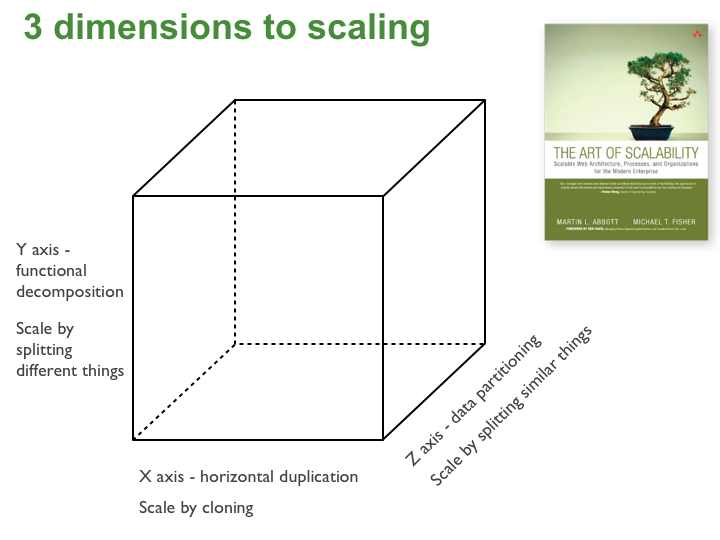
\includegraphics{img/ScaleCude.jpg}
\caption{Scaling Cube}
\end{figure}

Ahogy a képen is látható a meghatározó felbontási fogalmak, az adat
menti felbontás, a tetszőleges fogalom menti felbontás, illetve a
klónozás.

\subsubsection{Adat menti felbontás}\label{adat-menti-felbontuxe1s}

Az adat menti felbontás annyit tesz, hogy a szolgáltatásokat annak
megfelelően bontjuk fel, hogy milyen erőforrással dolgoznak, vagy
konkrétan egy adattal kapcsolatos összes funkciót egy helyen készítünk
el.

Példa: Erőforrás szerinti felbontás ha külön található szolgáltatás,
amivel az adatbázis műveleteket hajtjuk végre, és külön van olyan is,
ami csak a HTTP kéréseket szolgálja ki. Az egy adatra épülő módszernél
pedig alapul vehetünk egy olyan példát, ahol mondjuk egy szolgáltatás az
összes adminisztrátori funkciót látja el, míg más szolgáltatások a
más-más kategóriába eső felhasználók műveleteit hajtják végre.

Mivel a mikroszolgáltatások elve a hardvert is megosztja nem csak a
szoftvert, ezért az erőforrás szerinti szétválasztás kissé
értelmetlennek tűnhet, azonban a különböző platformok különbüző
erőforrásait megéri külön szolgáltatásként kezelni. Ha egy
mikroszolgáltatást tartunk arra, hogy az adatbázis kéréseket
kiszolgálja, akkor az adatbázis nem oszlik meg a szolgáltatások között.
Ennek ellenére pazarló lehet minden szolgáltatásnak saját adatbézist
fenntartani.

\subsubsection{Fogalmi felbontás}\label{fogalmi-felbontuxe1s}

A tetszőleges fogalom menti felbontás annyit tesz hogy elosztott
rendszert hozunk létre tetszőleges funkcionalitás szerint. Erre épít a
mikroszolgáltatás architektúra is, mivel a lényege pont az egyes
funkciók atomi felbontása.

Példa: Adott egy könyvtár nyilvántartó rendszere, és ezt akarjuk
fogalmanként szétvágni. Külön-külön lehet szolgáltatást csinálni a
keresésnek, indexelésnek, foglalásnak, kivett könyvek nyilvántartásának,
böngészésre, könyvek adatainak tárolására, és kiolvasására, és ehhez
hasonló funkciókra. Ezekkel a szétválasztásokkal a könyvtár működését
kis részekre bontottuk, és ezek egy-egy kis szolgáltatásként könnyen
elérhetők.

\subsubsection{Klónozás}\label{kluxf3nozuxe1s}

A harmadik módszer arra tér ki, hogy hogyan lehet egy architektúrát
felosztani, hogy skálázható legyen. Itt a klónozhatóság, avagy az egymás
melletti kiszolgálás motivál. Ez a mikroszolgáltatásoknál kell, hogy
teljesüljön, mivel adott esetben egy terheléselosztó alatt tudnunk kell
definiálni több példányt is egy szolgáltatásból. Azért szükséges a
skálázhatóság a mikroszolgáltatások esetén, mivel kevés hardver mellett
is hatékonyan kialakítható az architektúra, de könnyen lehet szűk
keresztmetszetet létrehozni, amit skálázással könnyen megkerülhetünk.

\subsection{Architektúrális mintákhoz való
viszonya}\label{architektuxfaruxe1lis-mintuxe1khoz-valuxf3-viszonya}

Mint korábban láthattuk vannak bizonyos telepítési módszerek, amik
mentén szokás a mikroszolgáltatásokat felépíteni. Van aki az
architektúrális tervezési minták közé sorolja a mikroszolgáltatás
architektúrát, de nem könnyű meghatározni, hogy hogyan is alkot önnáló
mintát. Nagyon sok lehetőség van a mikroszolgáltatásokban, és leginkább
más architektúrákkal együtt használva lehet hatékonyan és jól használni.

Nézzünk meg három felhasználható architektúrális mintát:

\subsubsection{Pipes and Filters}\label{pipes-and-filters}

A Pipes and filter architektúrális minta\citep{pipes-pattern} lényege,
hogy a funkciókra bontott architektúrát az elérni kívánt végeredmény
érdekében különböző módokon összekötjük. Ebben a módszerben az adat
folyamatosan áramlik az egyes alkotó elemek között, és lépésről lépésre
alakul ki a végeredmény. Elég olcsón kivitelezhető architektúrális
minta, mivel csupán sorba kell kötni hozzá az egyes szolgáltatásokat,
azonban nehezen lehet optimalizálni, és könnyen lehet, hogy olyan részek
lesznek a feldolgozás közben, amik hátráltatják a teljes folyamatot.

\subsubsection{Publisher/Subscriber}\label{publishersubscriber}

Egy másik, elosztott rendszerekhez kitallált minta a
publisher/subscriber\citep{pub-subscribed}, amely azon alapszik, hogy
egy szolgáltatásnak szüksége van valamilyen adatra vagy funkcióra, és
ezért feliratkozik egy másik szolgáltatásra. Ennek az lesz az eredménye,
hogy bizonyos szolgáltatások, bizonyos más szolgáltatásokhoz fognak
kötődni, és annak megfelelően fognak egymással kommunikálni, hogy milyen
feladatot kell végrehajtaniuk.

\subsubsection{Esemény alapú
architektúra}\label{esemuxe9ny-alapuxfa-architektuxfara}

Az esemény alapú architektúrákat\citep{event-driven-pattern} könnyen
kalakíthatjuk, ha egy mikroszolgáltatásokból álló rendszerben olyan
alkalmazásokat és komponenseket fejlesztünk ahol eseményeken keresztül
kommunikálnak az egyes elemek. Ezzel a nézettel olyan struktúrát lehet
összeépíteni, ahol a kis egységek szükség szerint kommunikálnak, és a
kommunikáció egy jól definiált interfészen keresztül történik.

\subsection{Eltérések a szolgáltatás orientált
architektúrától}\label{eltuxe9ruxe9sek-a-szolguxe1ltatuxe1s-orientuxe1lt-architektuxfaruxe1tuxf3l}

A mikroszolgáltatások a szolgáltatás orientált architektúrális minta
finomítása, mivel elsősorban szeparált egységeket, önműködő
szolgáltatásokat hoz létre, amik életképesek önmagukban is, és amennyire
lehet oszthatatlanok. A szolgáltatás orientált esetben viszont a meglévő
szolgáltatásainkat kapcsoljuk össze, ami akár egy helyen is futhat és
egyáltalán nem az atomicitás a lényege.

\subsection{Példák mikroszolgáltatásokat használó
alkalmazásokra}\label{puxe9lduxe1k-mikroszolguxe1ltatuxe1sokat-hasznuxe1luxf3-alkalmazuxe1sokra}

Amazon - minden Amazon-nal kommunikáló eszköz illetve az egyes funkciók
implementációja is szolgáltatásokra van szedve, és ezeket hívják az
egyes funkciók (vm indítás, törlés, mozgatás, stb.)

eBay - Különböző műveletek szerint van felbonva a funkcionalitás, és
ennek megfelelően külön szolgáltatásként érhető el a fizetés,
megrendelés, szállítási információk, stb.

NetFlix - A nagy terhelést elkerülendő bizonyos streaming
szolgáltatásokat átalakítottak, hogy a mikroszolgáltatás architektúra
szerint működjön.

Archivematica\citep{archivematica} - Egy Fájlkezelő rendszer, amiben
mikroszolgáltatásoknak megfelelően alakították ki a plugin-ként
használható funkciókat.

\section{Mikroszolgáltatások előnyei és
hátrányai}\label{mikroszolguxe1ltatuxe1sok-elux151nyei-uxe9s-huxe1truxe1nyai}

Ahogy minden architektúrális mintának, a mikroszolgáltatásoknak is
vannak előnyei\citep{microservices}, amik indokoltá teszik a minta
használatát, és vannak hátrányai\citep{micro-disadv}, amiket
mérlegelnünk kell a tervezés folyamán.

\subsection{Előnyök}\label{elux151nyuxf6k}

\subsubsection{Könnyű fejleszteni}\label{kuxf6nnyux171-fejleszteni}

Mivel kis részekre van szedve az alkalmazásunk, a fejlesztést akár több
csapatnak is ki lehet osztani, hogy az alkalmazás részeit alkossák meg,
hiszen önállóan is életképesek a szolgáltatások. Az egyes szolgáltatások
nem rendelkeznek túl sok logikával, így kis méretű könnyeb kezelhető
feladatokkal kell a csapatoknak foglalkozni.

\subsubsection{Egyszerűen
megérthető}\label{egyszerux171en-meguxe9rthetux151}

Egy szolgáltatás nagyon kis egysége a teljes alkalmazásnak, így könnyen
megérthető. Kevés technológia, és kevés kód áll rendelkezésre egy
szolgáltatásnál, így gyorsan beletanulhat egy új fejlesztő a munkába. A
dokumentáció, átláthatóság, illetve a hibák analizálása közben is jól
jön, hogy élesen elvállnak az egyes egységek.

\subsubsection{Könnyen kicserélhető, módosítható,
telepíthető}\label{kuxf6nnyen-kicseruxe9lhetux151-muxf3dosuxedthatuxf3-telepuxedthetux151}

A szolgáltatások önnálóan is működnek, így az azonos interfésszel
rendelkező szolgáltatásra bármikor kicserélhető, illetve módosítható ha
megmaradnak a korábbi funkciók. A szolgáltatás telepítése is egyszerű,
mivel csak kevés környezeti feltétele van annak, hogy egy ilyen kis
méretű progam működni tudjon. A fejlesztést nagyban segíti, hogy egy
korábbi verziójú programba plugin-szerűen be lehet integrálni az újonnan
fejlesztett részeket, mivel ez gyors visszajelzést ad a fejlesztőknek.
Ez a tulajdonsága a folytonos integrációt támogató eszközöknél is
előnyös, mivel könnyen lehet vele automatizált metodológiákat készíteni.

\subsubsection{Jól skálázható}\label{juxf3l-skuxe1luxe1zhatuxf3}

Mivel sok kis részletből áll az alkalmazásunk, nem szükséges minden
funkciónkhoz növelni az erőforrások allokációját, hanem kis
komponensekhez is lehet rendelni több erőforrást. Például egy számítási
felhőben, a teljesítményben látható változásokat könnyen és gyorsan
lehet kezelni, a problémát okozó funkció felskálázásval.

\subsubsection{Támogatja a kevert
technológiákat}\label{tuxe1mogatja-a-kevert-technoluxf3giuxe1kat}

Az egyik legnagyobb ereje ennek az architektúrának, hogy képes egy
alkalmazáson belül kevert technológiákat is használni. Mivel egy jól
definiált interfészen keresztül kommunikálnak a szolgáltatások, ezért
mindegy milyen technológia van mögötte, amíg ki tudja szolgálni a
feladatát. Ennek megfelelően el tudunk helyezni egy Linux-os
környezetben használt LDAP-ot, és egy Windows-os környezetben használt
Active Directory-t is, és minden gond nélkül használni is tudjuk őket az
interfésziek segítségével.

\subsection{Hátrányok}\label{huxe1truxe1nyok}

\subsubsection{Komplex alkalmazás alakul
ki}\label{komplex-alkalmazuxe1s-alakul-ki}

Mivel minden funkcióra saját szolgáltatást csinálunk, nagyon sok lesz az
elkülönülő elem, és a teljes alkalmazás egyben tartása nagyon nehéz
feladattá válik. Mivel fontos a szolgáltatások együttműködése, a sok
interfésznek ismernie kell egymást, és fenn kell tartani a
konzisztenciát minden szolgáltatással.

\subsubsection{Nehezen kezelhető az elosztott
rendszer}\label{nehezen-kezelhetux151-az-elosztott-rendszer}

A mikroszolgáltatások architektúra egy elosztott rendszert ír le, és
mint minden elosztott rendszer ez is bonyolultabb lesz a monolitikus
változatánál. Elosztott rendszereknél figyelni kell az adatok
konzisztenciáját, a kommunikáció plusz feladatot ad minden szolgáltatás
fejlesztőjének, és folyamatosan együtt kell működni a többi szolgáltatás
fejlesztőjével.

\subsubsection{Plusz munkát jelénthet az aszinkron üzenet
fogadás}\label{plusz-munkuxe1t-jeluxe9nthet-az-aszinkron-uxfczenet-fogaduxe1s}

Mivel egy szolgáltatás egyszerre több kérést is ki kell hogy szolgáljon
egyszerűbb ha aszinkron módon működik. Ezt azonban mindig le kell
implementálni, és az aszinkron üzenetek bonyolítják az adatok kezelését.
Az egyes szolgáltatások között könnyen lehetnek adatbázisbeli
inkonzisztenciák, mivel aszinkron működés esetén nem minden kiszolgált
kérésnek ugyan az a ritmusa. Ugyan nem megoldhatatlan feladat ezeket az
időbeli problémákat lekezelni, de plusz komplexitást hozhat be, amit egy
közös környezetben lock-olással könnyedén megoldhatnánk.

\subsubsection{Kód duplikátumok
kialakulása}\label{kuxf3d-duplikuxe1tumok-kialakuluxe1sa}

Amikor nagyon hasonló (kis részletben eltérő) szolgáltatásokat
csinálunk, megesik, hogy ugyan azt a kódot többször fel kell
használnunk, és ezzel kód, és adat duplikátumok keletkeznek, amiket le
kell kezelnünk. Nem nehéz találni olyan példát, ahol a létrehozás és
szerkesztés művelete megvalósítható ugyan külön szolgáltatásként,
viszont nehezíti a feladatot, hogy 2 külön adatbázist kéne módosítani az
ideális megvalósításban, és ezek konzisztenciáját fenn kéne tartani.

\subsubsection{Interfészek
fixálódnak}\label{interfuxe9szek-fixuxe1luxf3dnak}

A fejlesztés folyamán a szolgáltatásokhoz rendelt interfészek
fixálódnak, és ha módosítani akarunk rajta, akkor több szolgáltatásban
is meg kell változtatni az interfészt. Ennek a problémának a megoldása,
alapos tervezés, és sokszintű, bonyolult interfész struktúra
használatával megoldható.

\subsubsection{Nehezen tesztelhető
egészben}\label{nehezen-tesztelhetux151-eguxe9szben}

Mivel sok kis részletből rakódik össze a nagy egész alkalmazás, a
tesztelési fázisban kell olyan teszteket is végezni, ami a rendszer
egészét, és a kész alkalmazást teszteli. Egy ilyen teszt elksézítése
bonyolult lehet, és plusz feladatot ad a sok szolgáltatás külön-külön
fordítása, és telepítése is.

\subsection{Összehasonlítva a monolitikus
architektúrával}\label{uxf6sszehasonluxedtva-a-monolitikus-architektuxfaruxe1val}

A mikroszolgáltatás architektúra a monolitikus architektúra ellentetjei,
melyben az erőforrások központilag vannak kezelve, és minden funkció egy
nagy interfészen keresztül érhető el. A monolitikus architektúra
egyszerűen kiépíthető, könnyű tervezni és fejleszteni, azonban nehezen
lehet kicserélni, nem elég robosztus, és nehezen skálázható, mivel az
erőforrásokat közösen kezelik a funkciók.

Ezzel ellentétben a mikroszolgáltatás architektúrát ugyan nehezen lehet
megtervezni, hiszen egy elosztott rendszert kell megtervezni, ahol az
adatátviteltől kezdve az erőforrás megosztáson keresztül semmi sem
egyértelmű. A kezdeti nehézségek után viszont a későbbi továbbfejlesztés
sokkal egyszerűbb, mivel külön csapatokat lehet rendelni az egyes
szolgáltatásokhoz, és könnyen integrálhatók, kicserélhetők az alkotó
elemek. Mivel sok kis egységből áll, könnyebben lehet úgy skálázni a
rendszert, hogy ne pazaroljuk el az erőforrásainkat, és ugyanakkor a kis
szolgáltatások erőforrásokban is el vannak különítve, így nem okoz
gondot, hogy fel vagy le skálázzunk egy szolgáltatást. Ennek az a
hátránya, hogy le kell kezelni a skálázáskor a közös
erőforrásokat.(Például ha veszünk egy autentikációs szolgáltatást, akkor
ha azt fel skálázzuk, meg kell tartanunk a felhasználók listáját, így
duplikálni kell az adatbázist, és fenntartani a konzisztenciát) Ugyan
csak előnye a mikroszolgáltatás architektúrának, hogy különböző
technológiákat lehet keverni vele, mivel az egyes szolgáltatások
különböző technológiákkal különböző platformon is futhatnak.

\subsection{Archivematica}\label{archivematica}

Az Archivematica\citep{archivematica} egy nyílt forráskódú elektronikus
tartalom kezelő, ami tud kezelni különböző fájlokat, multimédiás
adatokat, illetve akármilyen szöveges tartalmat. Ez az alakmazás
alapvetően monolitikus architektúrára épül, azonban elkezdték
átalakítani a struktúráját mikroszolgáltatásokat használó
architektúrára. Ezt úgy kivitelezték, hogy a különböző plusz funkciókat
az eredeti alkalmazás plugin szerűen mikroszolgáltatásokból nyeri ki, és
ennek megfelelően a tovább fejlesztés is
megalapozott\citep{archivematica-wiki}.

\section{Technológiai
áttekintés}\label{technoluxf3giai-uxe1ttekintuxe9s}

Az integrációhoz olyan technológiákat\citep{micro-introPt1} lehet
használni, melyek lehetővé teszik az egyes szolgáltatások elkülönült
működését. Ahhoz, hogy jó technológiákat válasszunk, mindeképpen
ismernünk kell az igényeket, mivel a technológiák széles köre áll
rendelkezésünkre. Fontos szem előtt tartani pár általános érvényű
szabályt is\citep{micro-golden}, ami a mikroszolgáltatások helyes
működéséhez kell. Ezek pedig a következők:

\begin{itemize}
\tightlist
\item
  Modulárisan szétválasztani a szolgáltatásokat
\item
  Legyenek egymástól teljesen elkülönítve
\item
  Legyen jól definiált a szolgáltatások kapcsolata
\end{itemize}

A következő feladatokra kellenek technológiák:

\begin{itemize}
\tightlist
\item
  Hogyan lehet feltelepíteni egy önálló szolgáltatást? (telepítés)
\item
  Hogyan lehet összekötni ezeket a szolgáltatásokat? (automatikus
  környezet felderítés)
\item
  Hogyan lehet fenntartani, változtatni a szolgáltatások környezetét?
  (konfiguráció management)
\item
  Hogyan lehet skálázni a szolgáltatást? (skálázás)
\item
  Hogyan lehet egységesen használni a skálázott szolgáltatásokat? (load
  balance, konzisztencia fenntartás)
\item
  Hogyan lehet virtualizáltan ezt kivitelezni? (virtualizálás)
\item
  A meglévő szolgáltatásokat hogyan tartsuk nyilván? (service registy)
\item
  Hogyan figyeljük meg az alkalmazást működés közben (monitorozás,
  loggolás)
\end{itemize}

\subsection{Telepítési
technológiák}\label{telepuxedtuxe9si-technoluxf3giuxe1k}

A mikroszolgáltatásokat valamilyen módon létre kell hozni, egy hosthoz
kell rendelni, és az egyes elemeket össze kell kötni. A szolgáltatások
telepítéséhez olyan technológiára van szükség amivel könnyen elérhetünk
egy távoli gépet, és könnyen kezelhetjük az ottani erőforrásokat. Ehhez
a legkézenfekvőbb megoldás a Linux rendszerek esetén az SSH kapcsolaton
keresztül végrehajtott Bash parancs, de vannak eszközök, amikkel ezt
egyszerűbben és elosztottabban is megtehetjük.

\begin{itemize}
\item
  \textbf{Jenkins}\citep{jenkins}: A Jenkins egy olyan folytonos
  integráláshoz kifejlesztett eszköz, mellyel képesek vagyunk különböző
  funkciókat automatizálni, vagy időzítetten futtani. A Jenkins egy Java
  alapú webes felülettel rendelkező alkalmazás, amely képes bash
  parancsokat futtatni, Docker konténereket kezelni, build-eket
  futtatni, illetve a hozzá fejlesztett plugin-eken keresztül, szinte
  bármire képes. Támogatja a fürtözést is, így képesek vagyunk Jenkins
  slave-eket létrehozni, amik a mester szerverrel kommunikálva végzik el
  a dolgukat. A mikroszolgáltatás architektúrák esetén alkalmas a
  szolgáltatások telepítésére, és tesztelésére.
\item
  \textbf{ElasticBox}\citep{elasticbox}: Egy olyan alkalmazás, melyben
  nyilvántarthatjuk az alkalmazásainkat, és könnyen egyszerűen
  telepíthetjük őket. Támogatja a konfigurációk változását, illetve
  számos technológiát, amivel karban tarthatjuk a környezetünket
  (Docker, Puppet, Ansible, Chef, stb). Együtt működik különböző
  számítási felhő megoldásokkal, mint az AWS, vSphere, Azure, és más
  környezetek. Hasonlít a Jenkins-re, csupán ki van élezve a
  mikroszolgáltatás alapú architektúrák vezérlésére (Illetve fizetős a
  Jenkins-el ellentétben). Mindent végre tud hajtani ami egy
  mikroszolgáltatás alapú alkalmazáshoz szükséges, teljes körű
  felügyeletet biztosít. \citep{jenkins-elasticbox}
\item
  \textbf{Kubernetes}\citep{kubernetes}: A Kubernetes az ElasticBox egy
  opensource változata, ami lényegesen kevesebbet tud, azonban
  ingyenesen elérhető. Ez a projekt még nagyon gyerekcipőben jár, így
  nem tudom felhasználni a félév során.
\end{itemize}

Egyéb lehetőség, hogy a fejlesztő készít magának egy olyan szkriptet,
ami elkészíti számára a mikroszolgáltatás alapú architektúrát, és
lehetővé teszi az elemek dinamikus kicserélését (ad-hoc megoldás). Ennek
a megoldásnak a hátránya hogy nincs támogatva, és minden funkciót külön
kell implementálni. Sokkal nagyobb erőforrásokat emészthet fel mint egy
ingyenes, vagy nyílt forrású megoldást választani.

\subsection{Környezet felderítési
technológiák}\label{kuxf6rnyezet-felderuxedtuxe9si-technoluxf3giuxe1k}

Az egyes szolgáltatásoknak meg kell találniuk egymást, hogy megfelelően
működhessen a rendszer, azonban ez nem mindig triviális, így szükség van
egy olyan alkalmazásra, amivel felderíthetjük az aktív szolgáltatásokat.

\begin{itemize}
\tightlist
\item
  \textbf{Consul}\citep{consul}: A Hashicorp szolgáltatásfelderítő
  alkalmazása, amely egy kliens-szerver architektúrának megfelelően
  megtalálja a környezetében lévő szolgáltatásokat, és figyeli az
  állapotukat (ha inaktívvá válik egy szolgáltatás a Consul észre
  veszi). Ez az alkalmazás egy folyamatosan választott mester állomásból
  és a többi slave állomásból áll. A mester figyeli az alárendelteket,
  és kezeli a kommunikációt. Egy új slave-et úgy tudunk felvenni, hogy a
  consul klienssel kapcsolódunk a mesterre. Ha automatizáltan tudjuk
  vezényelni a feliratkozást, egy nagyon erős eszköz kerül a kezünkbe,
  mivel eseményeket küldhetünk a szervereknek, és ezekre különböző
  feladatokat hajthatunk végre.
\end{itemize}

A Consult leszámítva nem nagyon találtam olyan eszközt ami a nekem kellő
funkciókat tudta volna, főleg csak bizonyos szolgáltatásokhoz találtam
felderítő eszközt. A kézi megoldás itt is lehetséges, mivel saját
névfeloldás esetén a névfeloldó szervert használhatjuk az egyes
állomások felderítésére, vagy Docker-t használva a Docker hálózatok
elérhetővé teszik a szolgáltatásokat a futtató konténer hoszt nevével.

\subsection{Konfiguráció
management}\label{konfiguruxe1ciuxf3-management}

A telepítéshez és a rendszer állapotának a fenntartásához egy olyan
eszköz kell, amivel gyorsan egyszerűen végrehajthatjuk a
változtatásainkat, és ha valamit változtatunk egy szolgáltatásban, akkor
az összes hozzá hasonló szolgáltatás értesüljön a változtatásról, vagy
hajtson végre ő maga is változtatást.

\begin{itemize}
\item
  \textbf{Puppet}\citep{puppet}: Olyan nyílt forrású megoldás, amellyel
  leírhatjuk objektum orientáltan, hogy milyen változtatásokat akarunk
  elérni, és a Puppet elvégzi a változtatásokat. Automatizálja a
  szolgáltatás változtatásának minden lépését, és egyszerű, gyors
  megoldást szolgáltatat a komplex rendszerbe integráláshoz.
\item
  \textbf{Chef}\citep{chef}: A Chef egy olyan konfiguráció menedzsment
  eszköz ami nagy mennyiségű szerver számítógépet képes kezelni,
  fürtözhető, és megfigyeli az alá szervezett szerverek állapotát.
  Tartja a kapcsolatot a gépekkel, és ha valamelyik konfiguráció nem
  felel meg a definiált repectkönynek, (amiben definiálhatjuk az elvárt
  környezeti paramétereket) akkor változtatásokat indít be, és eléri,
  hogy a szerver a megfelelő konfigurációval rendelkezzen. Népszerű
  konfiguráció menedzsment eszköz, amit könnyedén használhatunk
  integrációhoz, illetve a szolgáltatások cseréjéhez, és
  karbantartásához.
\item
  \textbf{Ansible}\citep{ansible}: A Chef-hez hasonlóan képes
  változtatásokat eszközölni a szerver gépeken egy SSH kapcsolaton
  keresztül, viszont a Chef-el ellentétben nem tartja a folyamatos
  kapcsolatot. Az Ansible egy tipikusan integrációs célokra
  kifejlesztett eszköz, amelyhez felvehetjük a gépeket, amiken
  valamilyen konfigurációs változtatást akarunk végezni, és egy
  ``playbook'' segítségével leírhatjuk milyen változásokat kell
  végrehajtani melyik szerverre. Könnyen irányíthatjuk vele a
  szolgáltatásokat, és definiálhatunk szolgáltatásonként egy playbook-ot
  ami mondjuk egy fürtnyi szolgáltatást vezérel. Ez az eszköz hasznos
  lehet, ha egy szolgáltatásnak elő akarjuk készíteni a környezetet.
\item
  \textbf{SaltStack}\citep{saltstack}: A SaltStack nagyon hasonlít a
  Chef-re, mivel ez a termék is széleskörű felügyeletet, és konfiguráció
  menedzsmentet kínál számunkra, amit folyamatos kapcsolat
  fenntartással, és gyors kommunikációval ér el. Az Ansible-höz nagyon
  hasonlóan konfigurálható, szintén ágens nélküli kapcsolatot tud
  létesíteni, és a Chef-hez hasonlóan több 10 ezer gépet tud egyszerre
  karbantartani.
\end{itemize}

Minden konfigurációs menedzsment eszköznek megvan a saját nyelve, amivel
deklaratívan le lehet írni, hogy mit szeretnénk változtatni, és azokat a
program beállítja. Erre a feladatra nem nagyon érdemes saját eszközt
készíteni, mivel számos megoldás elérhető, és a megvalósítás komoly
tervezést, és fejlesztést igényel. Érdemes megemlíteni a Docker
konténerek adta lehetőséget, mivel a Docker konténerek gyorsan
konfigurálhatók, fejleszthetők, és a konténer képeken keresztül jól
karbantarthatók, így a konfiguráció menedzsment is megoldható velük. Ami
hiányzik ebből a megoldásból az a többi szolgáltatás értesítése a
változtatásról.

\subsection{Skálázási
technológiák}\label{skuxe1luxe1zuxe1si-technoluxf3giuxe1k}

A mikroszolgáltatás alapú architektúrák egyik nagy előnye, hogy az egyes
funkciókra épülő szolgáltatásokat könnyedén lehet skálázni, mivel egy
load balancert használva csupán egy újabb gépet kell beszervezni, és
máris nagyobb terhelést is elbír a rendszer. Ahhoz hogy ezt kivitelezni
tudjuk, szükségünk van egy terheléselosztóra, és egy olyan logikára, ami
képes megsokszorozni az erőforrásainkat. Számítási felhő alapú
környezetben ez könnyen kivitelezhető, egyébként hideg tartalékban
tartott gépek behozatalával elérhető. Sajnálatos módon általános célú
skálázó eszköz nincsen a piacon, viszont gyakran készítenek maguknak
saját logikát a nagyobb gyártók.

\begin{itemize}
\tightlist
\item
  \textbf{Elastic Load Balancer}\citep{elastic-load-balance}: Az Amazon
  AWS-ben az ELB avagy rugalmas terhelés elosztó az, ami ezt a célt
  szolgálja. Ennek a szolgáltatásnak az lenne a lényege, hogy segítse az
  Amazon Cloud-ban futó virtuális gépek hibatűrését, illtve egységbe
  szervezi a különböző elérhetőségi zónákban lévő gépeket, amivel
  gyorsabb elérést tudunk elérni. Mivel ez a szolgáltatás csupán az
  Amazon AWS-t felhasználva tud működni, nem megfelelő általános célra,
  azonban ha az Amazon Cloud-ban építjük fel a mikroszolgáltatás alapú
  architektúránkat, akkor erős eszköz lehet számunkra.
\end{itemize}

A skálázás egyik legegyszerűbb megvalósítása, hogy egy proxy szervert
felhasználva, valamilyen módon egységesen elosztjuk a kéréseket, és egy
saját monitorozó eszközzel figyeljük a terhelést (processzor terheltség,
memória, hálózati terhelés). Ha valamelyik érték megnő, egy ágenses vagy
ágens nélküli technológiával a virtualizált környezetben egy új példányt
készítünk a terhelt szolgáltatásból, és a proxy automatikusan megoldja a
többit. Nem tökéletes megoldát kapunk, azonban ez a legtöbb
felhasználási esetben megfelelőnek bizonyul.

\subsection{Terheléselosztás}\label{terheluxe9selosztuxe1s}

A mikroszolgáltatás alapú architektúrának egyik fontos eleme a terhelés
elosztó, vagy valamilyen fürtözést lehetővé tevő eszköz. Ez azért
fontos, mert egy egységes interfészt tudunk kialakítani a
szolgáltatásaink elérésére, és könnyíti a skálázódást a szolgáltatások
mentén.

\begin{itemize}
\item
  \textbf{HAProxy}\citep{haproxy} \citep{LB-haproxy}: Egy magas
  rendelkezésre állást biztosító, és megbízhatóságot növelő
  terheléselosztó eszköz. Konfigurációs fájlokon keresztül
  megszervezhetjük, hogy mely gépet hogyan érjünk el, milyen IP címek
  mely szolgáltatásokhoz tartoznak, illetve választhatóan round robin,
  legkisebb terhelés, session alapú, vagy egyéb módon osztja szét a
  kéréseket az egyes szerverek között. Ez az eszköz csak és kizárólak a
  HTTP TCP kéréseket tudja elosztani, de egyszerű, könnyen telepíthető,
  és könnyen kezelhető (ha nem dinamikusan változnak a fürtben lévő
  gépek, mert ha igen akkor szükséges egy mellékes frissítő logika is).
\item
  \textbf{ngnix}\citep{nginx}: Az Nginx egy nyílt forráskódú web
  kiszolgáló és reverse proxy szerver, amivel nagy méretű rendszereket
  kezelhetünk, és segít az alkalmazás biztonságának megörzésében. A
  kiterjesztett változatával (Nginx Plus) képesek lehetünk a
  terheléselosztásra, és alkalmazás telepítésre. Nem teljesen a proxy
  szerver szerepét váltja ki, de képes elvégezni azt.
\end{itemize}

A kézi megvalósítás gyakorlatilag egy kézileg implementált
terheléselosztó eszköz lenne, amihez viszont hálózati megfigyelés, és
routing szökséges, így nem javalott ilyen eszköz készítése.

\subsection{Virtualizációs
technológiák}\label{virtualizuxe1ciuxf3s-technoluxf3giuxe1k}

A mikroszolgáltatás alapú architektúrák kialakításánál nagy előnyt
jelenthet, ha valamilyen virtualizációt használunk fel a környezet
kialakításához. Virtualizált környezetben könnyebb a telepítés,
skálázás, és a monitorozás is egyszerűbb lehet.

\begin{itemize}
\item
  \textbf{Docker}\citep{docker}: Egy konténer virtualizációs eszköz,
  amelynek segítségével egy adott kernel alatt több különböző
  környezettel rendelkező, alkalmazásokat futtató környezetet hozhatunk
  létre. A Docker egy szeparált fájlrendszert hoz létre a gazda gépen,
  és abban hajt végre műveleteket. Készíthetünk vele előre elkészített
  alkalmazás környezeteket, és szolgáltatásokat, ami ideálissá teszi
  mikroszolgáltatás alapú architektúrák létrehozásánál. A Docker
  konténerek segítségével egyszerűen telepíthetjük, skálázhatjuk, és
  fejleszthetjük a rendszert.
\item
  \textbf{libvirt}\citep{libvirt}: Többféle virtualizációs
  technológiával egyűtt működő eszköz, amivel könnyedén irányíthatjuk a
  virtuális gépeket, és a virtualizálás komolyabb részét el
  absztrahálja. Támogat KVM-em, XEN-t, VirtualBox-ot, LXC-t, és sok más
  virtualizáló eszköt. Ezzel az eszközzel a környezet kialakítását
  szabhatjuk meg, tehát a hardveres erőforrások megosztásában nyújt nagy
  segítséget.
\item
  \textbf{kvm}\citep{kvm}: A KVM egy kernel szintű virtualizációs
  eszköz, amivel virtuális gépeket tudunk készíteni. Processzor szintjén
  képes szétválasztani az erőforrásokat, és ezzel szeparált
  környezeteket létrehozni. Virtualizál a processzoron kívül hálózati
  kártyát, háttértárat, grafikus meghajtót, és sok mást. A KVM egy nyílt
  forráskódú projekt és létrehozhatunk vele Linux és Windows gépeket is
  egyaránt.
\item
  \textbf{Akármilyen cloud}: Ha virtualizációról beszélünk, akkor adja
  magát hogy a számítási felhőket is ide értsük. Egy mikroszolgáltatás
  architektúrájú programot a legcélszerűbb valamilyen számítási felhőben
  létrehozni, mivel egy ilyen környezetnek definiciója szerint
  tartalmaznia kell egy virtualizációs szintet, megosztott
  erőforrásokat, monitorozást, és egyfajta leltárat a futó példányokról.
  Ennek megfelelően a mikroszolgáltatás alapú architektúra minden
  környezeti feltételét lefedi, csupán a szolgáltatásokat, business
  logikát, és az interfészeket kell elkészítenünk. Jellemzően a Cloud-os
  környezetek tartalmaznak terheléselosztást, és skálázási megoldást is,
  amivel szintén erősítik a szolgáltatás alapú architektúrákat. Ilyen
  környezet lehet az Amazon, Microsoft Azure, Google App Engine,
  OpenStack, és sokan mások.
\end{itemize}

Amennyiben nincs a kezünkben egy saját virtualizáló eszköz, a
virtualizálás kézi megvalósítása értelmetlen plusz komplexitást ad az
alkalmazáshoz.

\subsection{Szolgáltatás jegyzékek (service
registry)}\label{szolguxe1ltatuxe1s-jegyzuxe9kek-service-registry}

Számon kell tartani, hogy milyen szolgáltatások elérhetők, milyen címen
és hány példányban az architektúránkban, és ehhez valamilyen
szolgáltatás nyilvántartási eszközt\citep{service-registry-pattern}
\citep{micro-introPt3} kell használnunk.

\begin{itemize}
\item
  \textbf{Eureka}\citep{eureka-glance}: Az Eureka a Netflix fejlesztése,
  egy AWS környezetben működő terheléselosztó alkalmazás, ami figyeli a
  felvett szolgáltatásokat, és így mint nyilvántartás is megfelelő. A
  kommunikációt és a kapcsolatot egy Java nyelven írt szerver és kliens
  biztosítja, ami a teljes logikát megvalósítja. Együtt működik a
  Netflix álltal fejlesztett Asgard nevezetű alkalmazással, ami az AWS
  szolgáltatásokhoz való hozzáférést segíti. Ugyan ez az eszköz erősen
  optimalizált az Amazon Cloud szolgáltatásaihoz, de a leírás alapján
  megállja a helyét önállóan is. Mivel nyílt forráskódú, mintát
  szolgáltat egyéb alkalmazásoknak is.
\item
  \textbf{Consul}: Korábban már említettem ezt az eszközt, mivel abban
  segít, hogy felismerjék egymást a szolgáltatások. A kapcsolatot
  vizsgáló és felderítő logikán kívül tartalmaz egy nyilvántartást is a
  beregisztrált szolgáltatásokról, amiknek az állapotát is
  vizsgálhatjuk.
\item
  \textbf{Apache Zookeeper}\citep{zookeeper}: A Zookeeper egy
  központosított szolgáltatás konfigurációs adatok és hálózati adatok
  karbantartására, ami támogatja az elosztott működést, és a szerverek
  csoportosítását. Az alkalmazást elosztott alkalmazás fejlesztésre, és
  komplex rendszer felügyeletére és telepítés segítésére tervezték. A
  consulhoz hasonlóan működik, és a feladata is ugyan az.
\end{itemize}

Kézi megoldás erre nem nagyon van, csupán egy központi adatbázisban,
vagy leltár alkalmazásban elmentet adatokból tudunk valamilyen jegyzéket
csinálni, amihez viszont a szolgáltatások mindegyikének hozzá kell
férni. Könnyen konfigurálható megoldást kapunk, és tetszőleges adatot
menthetünk a szolgáltatásokról, de egyéb funkciók, mint az esemény
küldés és fogadás, csak bonyolult implementációval lehetséges.

\subsection{Monitorozás, loggolás}\label{monitorozuxe1s-loggoluxe1s}

Ha már megépítettük a mikroszolgáltatás alapú architektúrát, akkor meg
kell bizonyosodnunk róla, hogy minden megfelelően működik, és minden
rendben zajlik a szolgáltatásokkal. Ezekhez az adatokhoz többféle módon
és többféle eszközzel is hozzáférhetünk, mivel az alkalmazás hibákat egy
log szerver, a környezeti problémákat egy monitorozó szerver tudja
megfelelően megmutatni számunkra\citep{micro-service-monitoring}
\citep{microservice-monitoring}.

\begin{itemize}
\item
  \textbf{Zabbix}\citep{zabbix}: A Zabbix egy sok területen felhasznált,
  több 10 ezer szervert párhuzamosan megfigyelni képes, akármilyen
  adatot tárolni képes monitorozó alkalmazás, ami képes elosztott
  működésre, és virtuális környezetekben jól használható. Ágens nélküli
  és ágenses adatgyűjtésre is képes, és az adatokat különböző módokon
  képes megjeleníteni (földrajzi elhelyezkedés, gráfos megjelenítés,
  stb.). Nem egészen a mikroszolgáltatás alapú architektúrákhoz lett
  kialakítva, de egy elég általános eszköz, hogy felhasználható legyen
  ilyen célra is.
\item
  \textbf{Elasticsearch + Kibana\citep{kibana} +
  LogStash}\citep{logstash}: A Kibana egy ingyenes adatmegjelenítő és
  adatfeldolgozó eszköz, amit az Elasticsearch fejlesztett ki, és a
  Logstash pedig egy log server, amivel tárolhatjuk a loggolási
  adatainkat, és egyszerűen kereshetünk benne. Kifejezetten
  adatfeldolgozásra szolgál mind a két eszköz, és közvetlenül
  együttműködnek az Elasticsearch alkalmazással.
\item
  \textbf{Sensu}\citep{sensu}: A Sensu egy egyszerű monitorozó eszköz,
  amivel megfigyelhetjük a szervereinket. Támogatja Ansible Chef, Puppet
  használatát, és támogatja a plugin-szerű bővíthetőséget. A felülete
  letisztult, és elég jó áttekintést ad a szerverek állapotáról. Figyel
  a dinamikus változásokra, és gyorsan lekezeli a változásokkal járó
  riasztásokat. Ezek a tulajdonságai teszik a számítási felhőkben
  könnyen és hatékonyan felhasználhatóvá.
\item
  \textbf{Cronitor}\citep{cronitor} \citep{cron-monitoring}: Ez a
  monitorozó eszköz mikroszolgáltatások és cron job-ok megfigyelésére
  lett kifejlesztve, HTTP-n keresztül kommunikál, és a szologáltatások
  állapotát figyeli. Nem túl széleskörű eszköz, azonban ha csak a
  szolgáltatások állapota érdekel hasznos lehet, és segíthet a
  szolgáltatás jegyzék képzésében is.
\item
  \textbf{Ruxit}\citep{ruxit} \citep{ruxit-monitoring}: Egy számítási
  felhőben működő monitorozó eszköz, amivel teljesítmény monitorozást,
  elérhetőség monitorozást, és figyelmeztetés küldést végezhetünk. Az
  benne a különleges, hogy mesterséges intelligencia figyeli a
  szervereket, és kianalizálja a szerver állapotát, és a
  figyelmeztetéseket is követi. Könnyen skálázható, és használat alapú
  bérezése van. Ez a választás akkor jön jól, ha olyan feladatot szánunk
  az alkalmazásunknak, ami esetleg időben nagyon változó terhelést
  mutat, és az itt kapot riasztások szerint akarunk skálázni.
\end{itemize}

A monitorozás kézi megvalósítása egyszerűen kivitelezhető, ha van egy
központi adatbázisunk, amit minden szolgáltatás elér, és ebben az
adatbázisban a szolgáltatásokba ültetett egyszerű logika küldhet
adatokat, amit valamilyen egyszerű módszerrel megjelenítve, valamilyen
monitorozást érhetünk el. Ennek egyik előnye, hogy nem kell komplex
eszközt telepíteni mindenhova, és nem kell karban tartani, hátránya
viszont, hogy nehezen karbantartható, minden szolgáltatásra külön kell
elkészíteni, és a fenti megoldásokkal ellentétben a semmiből kell
kiindulni.

\section{Kommunikációs
módszerek}\label{kommunikuxe1ciuxf3s-muxf3dszerek}

A szolgáltatások közötti kommunikáció nincs lekötve de jellemző a
REST-es API, vagy a webservice-re jellemző XML alapú
kommunikáció\citep{rest-soap}.

\subsection{Technológiák}\label{technoluxf3giuxe1k}

A kommunikáció megtervezéséhez egy jó leírást olvashatunk az Nginx egyik
cikkében\citep{micro-communication}. Ez a cikk leírja, hogy fontos előre
eltervezni, hogy a szolgáltatások egyszerre több másik szolgáltatással
is kommunikálnak vagy sem, illetve szinkron vagy aszinkron módon
akarunk-e kommunikálni. A cikk kifejti, hogy az egyes technológiák
hogyan használhatók jól, és hogyan lehet várakoztatási sorral javítani a
kiszolgáláson.

\subsubsection{REST (HTTP/JSON):}\label{rest-httpjson}

A RESTful\citep{microservices-light} kommunikáció egy HTTP feletti
kommunikációs fajta, aminek az alapja az erőforrások megjelölése egyedi
azonosítókkal, és hálózaton keresztül műveletek végzése a HTTP
funkciókat felhasználva. Ez a módszer napjainkban nagyon népszerű, mivel
egyszerű kivitelezni, gyakorlatilag minden programozási nyelv támogatja,
és nagyon egyszerűen építhetünk vele interfészeket. Az üzenetek törzsét
a JSON tartalom adja, ami egy kulcs érték párokból álló adatstruktúra,
és sok nyelv támogatja az objektumokkal való kommunikációt JSON adatokon
keresztül (Sorosítással megoldható). Mikroszolgáltatások esetén az
aszinkron változat használata az előnyösebb\citep{rest-async}, mivel
ekkor több kérést is ki tudunk szolgálni egyszerre, és a
szolgáltatásoknak nem kell várniuk a szinkron üzenetek kiszolgálására.

\subsubsection{SOAP (HTTP/XML):}\label{soap-httpxml}

A szolgáltatás alapú architektúrákban nagyon népszerű a
SOAP\citep{soap}, mivel tetszőleges interfészt definiálhatunk, és le
lehet vele képezni objektumokat is. Kötött üzenetei vannak, amiket egy
XML formátumu üzenet ír le. Ebben az esetben nem erőforrásokat jelölnek
az URL-ek, hanem végpontokat, amik mögött implementálva van a
funkcionalitás. Ennek a kommunikációs módszernek az az előnye, hogy jól
bejáratot, széleskörben használt technológiáról van szó, amit jól lehet
használni objektum orientált nyelvek közötti adatátvitelre. Hátránya,
hogy nagyobb a sávszélesség igénye, és lassabb a REST-es megoldásnál.
Létezik szinkron és aszinkron megvalósítása is és mivel ez a
kommunikációs fajta is HTTP felett történik, a REST-hez hasonló okokból
az aszinkron változat a célszerűbb.

\subsubsection{Socket (TCP):}\label{socket-tcp}

A socket\citep{socket} kapcsolat egy TCP feletti kapcsolat, ami egy
folytonos kommunikációs csatornát jelent az egyes szolgáltatások között.
Ez azért lehet előnyös, mert a folytonos kapcsolat fix útvonalat és fix
kiszolgálást jelent, amivel gyors és egyszerű kommunkácót lehet
végrehajtani. A három technológia közül ez a leggyorsabb és a legkisebb
sávszélességet igénylő, azonban nincs definiálva az üzenetek formátuma
(protokollt kell hozzá készíteni), és az aszinkron elv nem
összeegyeztethető vele, így üzenetsorokat kell létrehozni a párhuzamos
kiszolgáláshoz. Indokolt esetben sok előnye lehet egy
mikroszolgáltatásokra épülő struktúrában is, azonban általános esetben
nem igazán használható kommunikációs eszköz.

\subsection{Interfészek}\label{interfuxe9szek}

A korábban említett Nginx-es cikk kitért arra is, hogy az interfészek
megalkotása milyen gondokkal járhat, és mi az előnye, hogyan lehet úgy
megtervezni őket, hogy ne legyen sok gondunk velük.

Az interfészeket úgy kell megtervezni, hogy könnyen alkalmazhatók
legyenek, képesek legyünk minden funkciót teljes mértékben használni, és
később bővíthető legyen (visszafelé kompatibilis). Erre egy megoldás a
RESTful technológiáknál a verziózott URL-ek használata, amivel implicit
módon megmondhatjuk, hogy melyik verziójú interfészre van szükségünk
éppen. Ha rosszul tervezzük meg az interfészek struktúráját, és nem
készítjük fel a szolgáltatásokat egy lehetséges interfész változtatásra,
akkor könnyen lehet, hogy nagy mennyiségű plusz munkát adunk a
fejlesztőknek, akiknek minden hívást karban kell tartaniuk.

\chapter{Minta alkalmazás}\label{minta-alkalmazuxe1s}

\begin{figure}[H]
\centering
\includegraphics{img/microservices.png}
\caption{Microservices}
\end{figure}

\section{Alkalmazás leírás:}\label{alkalmazuxe1s-leuxedruxe1s}

Az alkalmazás, amin ketesztül a mikroszolgáltatások működését bemutatom,
egy könyvesbolt webárúháza lesz, ami rendelkezik egy webes felülettel. A
felhasználó be tud jelentkezni a felületre, és tud könyveket vásárolni
magának a webes nyilvántartásból.

\section{Szolgáltatások:}\label{szolguxe1ltatuxe1sok}

A szolgáltatások meghatározásánál elsőnek azt vettem alapul, hogy milyen
feladatokat kell teljesítenie a rendszernek, majd az erőforrásokat
vettem alapul.

A könyvesbolthoz tartozóan a következő tevékenységeket határoztam meg:

\begin{itemize}
\tightlist
\item
  \textbf{Bejelentkezés}: Felhasználó felületen történő authentikálása.
\item
  \textbf{Böngészés}: Felhasználó láthatja mi van a raktáron.
\item
  \textbf{Vásárlás}: Felhasználó valamit a saját nevére ír, megvásárol.
\end{itemize}

A könyveket egy adatbázisban tárolom a megrendelésekkel együtt, és egy
proxy-t is készítettem, hogy könnyen skálázható legyen bármely funkció.

\begin{itemize}
\tightlist
\item
  \textbf{Adabtbázis}: Tartalmazza a tárolt könyveket, autentikációs
  adatokat, és vezeti a vásárlások naplóját.
\item
  \textbf{Proxy}: Minden szolgáltatást elérhetővé tesz egy közös
  interfészen keresztül, és skálázhatóvá teszi a szolgáltatásokat.
\end{itemize}

Ezekből a feladatokból a következő szolgáltatásokat lehet elkészíteni:

\begin{itemize}
\tightlist
\item
  \textbf{Felület kiszolgálása}: Egy web kiszolgáló alkalmazása, amin
  keresztül elvégezhetők a különböző műveletek, mint a bejeletkezés,
  vagy vásárlás. Ez a felület magába foglalja a böngészést lehetővé tevő
  szolgáltatást is, mivel szorosan ehhez a funkcióhoz tartozik. Egy
  másik megvalósítás lehetne, hogy a különböző vetületekhez tartozó
  információt egy-egy szolgáltatás adja vissza, azonban ez túl nagy
  komplexitást eredményezne, így az elöbbi megoldásnál maradtam.
\item
  \textbf{Authentikációs szolgáltatás}: A bejelentkezni szándékozó
  felhasználó adatait ellenőrzi, és hibás bejelentkezés esetén hibát
  dob. Az adatbázissal kommunikál, és ellenőrzi, hogy a felhasználónak
  van-e bejegyzése az adatbázisban.
\item
  \textbf{Vásárlási szolgáltatás}: A böngészés közben kiválasztott
  könyveket lefoglalja a raktári készletből. Csökkenti az adatbázisban a
  készlet tartalmát, és létrehoz egy új bejegyzést a vásárlások
  adattáblájában, ami tartalmazza a vásálás adatait. Ha túl sokat akar
  venni a felhasználó, vagy nem létező könyvből akar vásárolni, akkor
  hibajelzést küldök.
\item
  \textbf{Adatbázis szolgáltatás}: Ez a szolgáltatás tartalmazza a
  raktár tartalmát, a vásárlási naplót, és a bejelentkezési adatokat.
  Mivel a legtöbb adatbázis kezelő távolról elérhető, és fürtözési
  lehetőségeket is nyújt, ezért ehhez a szolgáltatáshoz nem szükséges
  mögöttes logika. Az interfésze az adatbázist kezelő eszköz interfésze
  (pl.: MySQL szerver, és SQL nyelvű interfész.).
\item
  \textbf{Terhelés elosztó szolgáltatás}: Ez a szolgálatatás a
  skálázhatóságot segíti, és egy egységes interfész kialakításában
  segít. Tartalmaz egy proxy kiszolgálót, és egy konfigurációs fájlt,
  amit az infrastruktúra változásával bővítünk (pl.: HAProxy, és a hozzá
  tartozó konfigurációs fájl). Nehéz kérdés lehet egy új szolgáltatás
  beiktatása, mivel a proxy szerver interfésze változna meg tőle, így
  ennek a szolgáltatásnak a többivel együtt kell változnia.
\end{itemize}

\section{Értékelés}\label{uxe9rtuxe9keluxe9s}

Az alkalmazás kellően egyszerű, hogy rövid idő alatt implementálni
lehessen, és alkalmas rá, hogy a fejlesztés során használt folytonos
integrációra épülő feladatokat bemutassam rajta.

A tervben azért szerepelnek külön az adatbázis és a proxy szoláltatások,
mivel túl bonyolulttá, és feleslegesen erőforrás igényessé tenné az
alkalmazást, ha minden szolgáltatás saját adatbázissal rendelkezne és a
saját skálázhatóságát is menedzselné. Van néhány bottleneck
szolgáltatás, mint a web kiszolgáló, és az adatbázis szerver, viszont
egy olyan változat, melyben ez nem áll fenn, nagyságrendekkel több idő
lett volna elkészíteni, így a diplomaterv során ezzel nem foglalkoztam.

\chapter{Implementáció és kapcsolódó
nehézségek}\label{implementuxe1ciuxf3-uxe9s-kapcsoluxf3duxf3-nehuxe9zsuxe9gek}

\section{Minta alkalmazás
implementációja}\label{minta-alkalmazuxe1s-implementuxe1ciuxf3ja}

A minta alkalmazás megvalósításához \emph{Docker} konténereket
használtam, hogy a saját laptopomon, vagy egy dedikált gépen is meg
tudjam oldani az elosztott alkalmazást, mivel így kevés erőforrással is
meg tudtam csinálni amit akartam. A kommunikációra kiválasztott módszer
a \emph{REST}-es kommunikáció lett, mivel egy széles körben használt
megoldás, és rengeteg nyelv támogatja. A szolgáltatások jegyzéséhez
\emph{Consult} használtam, ami az utóbbi években sokat fejlődött, és
elég átfogó funkcionalitást nyújt számomra.

\subsection{Szolgáltatások megvalósítása Docker
konténerekben}\label{szolguxe1ltatuxe1sok-megvaluxf3suxedtuxe1sa-docker-kontuxe9nerekben}

A mikroszolgáltatások egyik legnagyobb előnye, hogy különböző
platformokat és programozási nyelveket használhatunk az architektúrában
különösebb probléma nélkül. Ezt a Docker-el úgy oldottam meg, hogy
Centos és Ubuntu disztribúciójú környezeteket, és PHP, Python, Java,
illetve Bash szkripteket használtam.

A szolgáltatásokhoz tartozó Docker konténerek:

\begin{itemize}
\tightlist
\item
  \textbf{Adatbázis}: Az alapja egy \emph{`mysql'} nevezetű konténer,
  ami tartalmaz egy lightweight Ubuntu-t és benne telepítve egy mysql
  szervert. Ezt a konténert egy inicializáló szkripttel egészítettem ki,
  ami elkészítette az alap adatbázist.
\item
  \textbf{Terheléselosztó}: A terheléselosztást \emph{HAProxy}-val
  oldottam meg, amit egy Ubuntu konténerre alapoztam. Létezik egy olyan
  Docker konténer, ami kifejezetten HAProxy mikroszolgáltatásnak van
  nevezve, azonban ez a konténer nehezen használható, és a szolgáltatás
  újraindítása is el lett rontva benne, így egyszerűbbnek láttam egy
  saját megvalósítást használni.
\item
  \textbf{Webkiszolgáló}: A weboldal kiszolgálását egy \emph{`httpd'}
  nevű lightweight konténer szolgálja ki amiben egy apache webkiszlgáló
  van. Ezt kiegészítettem néhány \emph{PHP} szkripttel, ami kiszolgálja
  a kéréseket. Ezt a konténert terveztem úgy, hogy a kéréseket ő
  szolgálja ki és ezen a szolgáltatáson keresztül érhető el a többi
  funkcionalitása.
\item
  \textbf{Authentikáció}: Egyszerű Ubuntu konténer, ami fel van szerelve
  \emph{Python}-nal, és a \emph{MySQLdb} Python könyvtárral. Ezen felül
  tartalmaz egy REST-es kiszolgálót, amin keresztül elérhető a
  szolgáltatás. Az authentikáció egyszerű adatbázis alapú azonosítás,
  amit kódolatlanul tárolunk a MySQL adatbázisunkban. Éles változatban
  természetesen ez nem elegendő.
\item
  \textbf{Vásárlás}: Centos konténer alapú környezet, amiben \emph{Java}
  lett telepítve, és egy webes REST API-n keresztül érhetjük el a
  szolgáltatását. A konténer webes szolgáltatását \emph{Ngnix}
  segítségével tettem elérhetővé. Sajnos a félév során változott a
  Centos alap image repository-ja, és használhatatlanná tette a
  szolgáltatást, mivel az Ngnix szolgáltatást többé nem tudtam
  elindítani. Erről a problémáról bövebben a `Nehézségek, megoldás
  értékelése' fejezetben írok.
\end{itemize}

\section{Szolgáltatás felismerés
megoldásai}\label{szolguxe1ltatuxe1s-felismeruxe9s-megolduxe1sai}

A szolgáltatások magukban nem sokat érnek, viszont nem tudnak együtt
működni ha nem ismerik egymás elérési útvonalát. Ahhoz, hogy a megfelelő
helyre érkezzenek be az üzenetek, valamilyen névfeloldásra van szükség,
amely képes irányítani a kéréseket a komplex architektúrában. Egyik
lehetőség, hogy a Docker álltal szolgáltatott személyre szabott
válózatot használjuk, és jól elnevezett konténereket hozunk létre. Egy
másik lehetőség a Consul használata, ami nyilvántartja a beregisztrált
végpontokat, és elérhetővé teszi egymás számára. A névfeloldáshoz Consul
esetében kis trükkre van szükség, de nem olyan nagy feladat. Ugyan a
diplomaterv keretei között csak ezt a két módszert vizsgáltam meg,
azonban lehetséges saját névfeloldó szervert karbantartani, vagy egy jól
felügyelt környezetben konténereket indítani, mint az Amazon AWS
Cloud-ban, ami támogatja ezeket a funkciókat.

\subsection{Kapcsolatok építése
Docker-el:}\label{kapcsolatok-uxe9puxedtuxe9se-docker-el}

Ahogy korábban már említettem lehetőség van a Docker legújabb verzióiban
megadni, hogy ez egyes konténerek milyen néven és milyen hálózaton
keresztül érhető el a többi konténer. A név beállításához a docker run
parancs \texttt{-\/-hostname} paraméterét használhatjuk, míg a hálózat
definiálásához előbb létre kell hozni egy új Docker hálózatot

\begin{verbatim}
  docker network create bookstore
\end{verbatim}

amire a konténerek tudnak csatlakozni a \texttt{-\/-net} kulcsszóval.
Ennek segítségével elérhető, hogy nagyon egyszerűen és egy eszköz
felhasználásával képesek legyenek látni egymást a szolgáltatások,
viszont egy nagy hátulütője van a megoldásnak, mégpedig az, hogy egy
gépen kell futnia az összes alkalmazásnak. Másik hátránya ennek a
megoldásnak, hogy a konténerek közül csak egynek lehet olyan nevet adni,
ami a szolgáltatásra utal (egyszerre csak egy konténernek lehet mondjuk
webserver neve), és éppen ezért a skálázáshoz egy saját logikát kell
építeni. Mivel ez egy mikroszolgáltatásokra épülő architektúránál közel
sem ideális, így ez csupán fejlesztési, és reprezentatív jelleggel
használható.

\subsection{Kapcsolatok építése
Consul-al:}\label{kapcsolatok-uxe9puxedtuxe9se-consul-al}

A Consul alkalmazást korábbi félév folyamán használtam már, teljesítmény
mérések futtatására Docker konténerben, így megpróbáltam átültetni a
logikát a jelenlegi mikroszolgáltatásokat biztosító architektúrába. A
gondot az okozta, hogy a Consul alkalmazásnak szükséges egy fix pont,
így alkottam egy logikát, melyben minden szolgáltatás önálló szerverként
funkcionál, és az összes szolgáltatás próbál csatlakozni az alháózatban
lévő végpontokra. Ennek az az eredménye, hogy minden csatlakozó szerver
egy új lehetőséget biztosít, és lassan de biztosan kiépül a Consul
hálózat.

Ez a megoldás magában nem elegendő, hogy felismerjék egymást a
szolgáltatások, így fel kellett használnom a Consul Template nevezetű
technikát, amiben a proxy beállításokban az egyes szolgáltatásokhoz
tartozó elemeket egy bejegyzés alá rendelem. Ennek megfelelően a proxy-n
keresztül minden szolgáltatás minden más szolgáltatást elér, ás a
skálázás esetán a proxy megoldja az új elem lekezelését. Mivel ez a
megoldás sokkal robosztusabb a Docker alapúnál, ezért ezt használtam a
végső programban.

\section{Nehézségek, megoldás
értékelése}\label{nehuxe9zsuxe9gek-megolduxe1s-uxe9rtuxe9keluxe9se}

Sajnálatos módon egy ilyen összetett, és elágazó rendszer esetén gyakran
ütközünk problémákba, és ezeket a gondokat leggyakrabban nem is a saját
fejlesztésünk, hanem a használt eszküzük okozzák. Erre a célra hasznos
lehet fenntartani a folytonos integrációt támogató eszközben egy eszköz
konzisztenciát, és visszafelé kompatibilitást tesztelő részt
fejleszteni, illetve lassan, és megfontoltan váltani az új
eszközverzióknál.

\subsection{Nehézségek a Docker
használatával}\label{nehuxe9zsuxe9gek-a-docker-hasznuxe1latuxe1val}

A diplomaterv elkészítése során számtalanszor futottam olyan hibába,
amit a Docker konténerek használata okozott. Volt olyan, hogy az alapul
szolgáló image készítésekor nem volt megfelelő a repository, és eltűntek
csomagok amikre szükségem lett volna, hol a futó konténerek álltak le
minden ok nélkül. A Docker fejlesztése közben sajnálatos módon nem
gondoltak a visszafele kompatibilitásra, és minden új verzióban van
valamilyen meglepetés, ami nem úgy működik, mint a korábbiban. Találtam
egy cikket\citep{docker-is-bad}, ami leírja a legtöbb problémát, amivel
Docker konténerek használata közben találkozhatunk, viszont nem igazán
van alternatív lehetőség.

Az egyik legnagyobb probléma amivel találkoztam, az a Centos alapú
konténerek esetében jelentkezett. Ez a probléma az volt, hogy a Centos
alap image megváltozott, és onnantól kezdve nem lehetett használni benne
az Nginx szolgáltatást, vagy akármyilen szolgáltatást. A Docker
konténerekben használt programok megváltoztak, és a build során történt
frissítés lehetetlenné tette a szolgáltatás működését. Megoldásként
átálltam egy Ubuntu alapú image-re, mivel abban nem jelentkezett ilyen
jellegű hiba.

\subsection{Nehézségek a Consul
használatával}\label{nehuxe9zsuxe9gek-a-consul-hasznuxe1latuxe1val}

A Consul használatához hozzászoktam már a korábbi félévek során, de az
újítások miatt kicsit át kellett gondolnom a használatot. Eleinte
megpróbáltam használni az önálló laboratórium során használt
szkriptemet, de valamilyen szintaktikai hibára panaszkodott, és nem
tudtam használni azt a változatot. Az én megérzésem az, hogy az
események küldésében történt valami, mivel látszólag a Docker-el
ellentétben a Consul visszafelé kompatibilis, és a szerver építés nem
változott. Sajnálatos módon elég sok időt emésztett fel egy új változat
elkészítése, ami végül sokkal hibatűrőbb lett, mint elődje, és nem csak
egy fix ponton keresztül lehet elérni a többi Consul klienst. Egy másik
változtatás lett, hogy minden végpont szerverként funkcionál, így ha
kiesik valamelyik szerver, a Consul hálózat nem szakad meg, és nem kell
újra építeni.

A Consul template egy új fejlesztése a Hashicorp-nak, és a honlapon ad
is pár mintát a fejlesztő cég, azonban nincs kiélezve a valóságra, így
kénytelen voltam más forrásokból megtudni, hogy hogyan célszerű
használni a Consul Template-et HAProxy-val. Az előző félévben események
küldésével oldottam ezt meg, viszont ez az új funkció sokkal
ígéretesebbnek tűnt.

\subsection{Váratlan meglepetések}\label{vuxe1ratlan-meglepetuxe9sek}

Ugyan a legnagyobb meglepetést a Docker okozta az image
inkonzisztenciájával, de ettől függetlenül volt néhány apróbb
meglepetés, ami a fejlesztést visszavetette. Egy ilyen meglepetés
például, hogy a Docker konténerekben beállított hosts fájl tartalma már
nem az mint korábban, és ezen keresztül nem látják egymást a
konténerekek. A HAProxy-val kapcsolatban ez előző félévhez képest nem
történt semmi, azonban a felhasznált verzió változhatott, mivel sem az
indító szkript, sem a konfigurációs fájl nem ott volt megtalálható, mint
az előző félévben.

Ami a MySQL-t illeti a Docker konténerekben való használata nem igazán
támogatott dolog, mivel nem kéne kritikus adatokat használni a
konténerekben, de az előző félévhez képest változott a csomag, mivel a
konténer buildelésénél egy olyan hiba merült fel, hogy a csomag kiakadt,
amikor a felhasználó nevet és jelszót kérte a telepítő. Ezt egy egyszerű
módosítás megoldotta, de nagyon sok idő volt rájönni, mivel is van a
baj. Ami az adatbázist illeti, nem csak a csomag de a működés és a hozzá
tartozó authentikáció is megváltozott, mivel az előző félévben képes
voltam jelszó nálkül használni a felhasználót, addig ebben a félévben
kötelező volt megadnom valamit, ami az összes szolgáltatás
változtatásával járt.

\subsection{Értékelés}\label{uxe9rtuxe9keluxe9s-1}

\subsubsection{Komponensek}\label{komponensek}

A minta alkalmazás főbb komponensei a mikroszolgáltatások elve szerint
lettek szétválasztva, azonban az adatbázis külön szolgáltatásként
kezelése nem teljesen ezt a metodológiát követi. A praktikusság és
erőforrás kezelés szempontjából sokkal jobb megoldást kaptam, mint ha az
össze szolgáltatás önálló adatbázissal rendelkezne, de lehet, hogy még
jobb lett volna egy szolgáltatásokon kívül elhelyezkedő adatbázis
szerver. Ami az authentikációt illeti, lehetséges, hogy jobban jártam
volna egy szolgáltatásonkénti ellenörzéssel, mivel ha kiveszem az
authentikációt vezérlő szolgáltatást, az egész alkalmazás veszélynek
lesz kitéve. Természetesen más megközelítésből ez a tervezés éppen jó,
hiszen az authentikálás funkcióját csak egy szolgáltatás végzi, és így
plugin-szerűen kivehető, vagy berakható.

\subsubsection{Kommunikáció}\label{kommunikuxe1ciuxf3}

Ami a Rest kommunikációt illeti, teljesen megfelelt a célnak, és könnyen
egyszerűen tudtam vele változtatni az interfészeket, és nagyon egyszerű
volt a kiszolgáló alkalmazások elkészítése is. Ha cél lett volna más
kommunikációs technológiák bemutatása is, akkor sokkal nehezebb
feladatom lett volna, mivel a kevert Rest-es és XML alapú, vagy socket
kommunikáció, komoly többlet fejlesztés okozott volna, illetve a
struktúrát is átrajzolta volna.

\subsubsection{Fejlesztési élmény}\label{fejlesztuxe9si-uxe9lmuxe9ny}

A minta alkalmazás fejlesztése során nem használtam semmilyen folytonos
integrációt támogató eszközt, se semmilyen automatizált módszert, ami
ellenőrizte volna a munkámat. Sajnos ez nagyon megnehezítette a
fejlesztést, mivel minden alkalommal külön meg kellett győződnöm arról,
hogy az alkalmazás minden eleme külön elkészíthető, és a létrehozott
alkalmazás is jól használható, illetve az interfészek is jól működnek.
Ha lett volna valamilyen automatizált módszer, ami a kód szintaktikáját
folyamatosan figyelte volna minden változtatáskor, vagy lett volna
valamilyen logika, ami megpróbálta volna összerakni az alkalmazást, és
funkció tesztek alapján megmondta volna, hogy jó-e amit csinálok, akkor
sokkal gyorsabban is haladhattam volna. A félév során több Docker-es
problémába is beleütköztem, és volt, hogy csak órák alatt jöttem rá,
hogy a Docker konténer a hibás. Ezt egy egyszerű konzisztencia
ellenőrzés elkaphatta volna és percek alatt meglett volna a hibaok.

\section{Automatizálás}\label{automatizuxe1luxe1s}

Mint azt az előző fejezetben kifejtettem, sok haszna lehet, ha van
valamilyen automatizált tesztelő, és integráló eszköz a
mikroszolgáltatás alapú infrastruktúránk támogatására. Ahhoz, hogy
teljes mértékben támogatni tudjuk a fejlesztés minden aspektusát,
különböző módszereket, és alkalmazásokat tudunk használni.

\subsection{Kódolás tesztelése}\label{kuxf3doluxe1s-teszteluxe9se}

Mivel folyamatosan készül új kód, és ennek a kódnak minőségileg és
tartalmilag is helyesnek kell lennie, teszteket készíthetünk, amik még
kezdeti fázisban elkapják a stillisztikai és kódolási hibákat. Ilyen
lehet például a Git verzió kezelő esetén egy olya hook, ami leellenőrzi
egy kód ellenőrzővel a szintaktikát (mint például Python kód esetén
pylint alkalmazást futtatva), majd megvizonyosodik a szemantikáról is
egy gyors unit teszt futtatással. Ez a megoldás egy azonnali választ ad
a fejlesztőnek, hogy jól csinálja amit csinál, és vissza tartja a hibás
kódrészleteket.

\subsection{Funkcionalitás
tesztelése}\label{funkcionalituxe1s-teszteluxe9se}

Mivel minden konténer önálló alkalmazás, így az egyes alkalmazásokat
magukban is lehet tesztelni, és lefedve az összes lehetséges
felhasználási módot funkció teszteket futtathatunk. Ez a megoldás
szintén lehet valamilyen verzió kezelőhöz kötve, vagy egy automatozáló
eszközt felhasználva, tudunk eseményekre teszteket futtatni. Ez főleg
abban segít, hogy ne kelljen értelmetlenül időt pazarolni a
mikroszolgáltatás buildelésére, illetve az integrációra, ha meg tudjuk
mondani, hogy nem megfelelő a szolgáltatás alapja.

\subsection{Interfész tesztek}\label{interfuxe9sz-tesztek}

Ez egy nehezebb kérdés, de hasznos lehet, ha valamilyen módon le tudjuk
ellenőrizni, hogy a szolgáltatások közötti interfészek konzisztensek-e a
régiekkel, és használhatók-e rendesen. Ez leginkább csak akkor
kivitelezhető, ha jó leíró fájlokkal tudjuk megmondani, hogy milyen
intefészek vannak az alkalmazásban. Ezzel a teszttel a cél az lenne,
hogy ne tudja a fejlesztő csapatok közül egy se elrontani a többi
szolgáltatás interfészével az konzisztenciát. Az automatizált megoldás a
kódolás tesztek mellett futhat, hiszen erről is egy gyors visszajelzés a
legcélravezetőbb.

\subsection{Teljes működés
tesztje}\label{teljes-mux171kuxf6duxe9s-tesztje}

Ez a legbonyolultabb művelet, amivel meg tudjuk mondani, hogy mindaz
amit fejlesztettünk működik, együttműködik a többi szolgáltatással, és
pontosan úgy működik ahogy szeretnénk. Sokan a pipeline terminológiát
használják az ehhez hasonló funkcióhoz, ami annyit jelent, hogy a
beadott adatokra egy kimeneti artifactot kapunk. A legáltalánosabb
módszer, amit szinte mimnden felhasználásra rá lehet húzni, az egy
buildelési folyamattal indul (építés), majd összeállít egy tesztelhető
környezetet (telepítés), és végül a funkció teszteket, vagy integrációs
teszteket (teszt) futtata. Ehhez a tesztelési stílushoz már kell egy
olyan eszköz, amivel összehangoltan fel tudjuk építeni a teljes
folyamot, és meg tudjuk oldani, hogy a végeredmény és a köztes
információk elérhetők legyenek. Egy ilyen eszköz a folytonos integrációt
támogató Jenkins, amiben könnyedén össze lehet állítani a megfelelő
folyamot, hívási struktúrát. Természetesen ha szeretnénk csinálhatunk
saját megoldást is, ami szkripttekkel és időzítő eszközökkel (például
Bash és Cron) szintén megoldható.

\section{Folytonos integrációs lépések
tervezése}\label{folytonos-integruxe1ciuxf3s-luxe9puxe9sek-tervezuxe9se}

Mielőtt nekikezdtem volna a konkrét implementációnak, megnéztem, hogy
miket is kéne végrehajtanom a saját pipeline-om futtatása során.

\begin{enumerate}
\def\labelenumi{\arabic{enumi}.}
\tightlist
\item
  \textbf{Teszt alkalmazás build-elése}: Gyakran van szükség a
  szolgáltatást futtató fájlok és egyéb tartalmak fordítására (C, Java,
  bináris kép fájlok frodítása), és ezeket a forrásokat könnyedén
  elkészíthetjük automatizáltan is, mielőtt a környezetet
  összeépítenénk.
\item
  \textbf{Teszt architektúra telepítése}: Az egyes szolgáltatásokat egy
  felügyelt környezetbe helyezve valamilyen környezeti konfigurációval
  együtt telepíthetjük (esetünkben Docker konténerekbe csomagolhatjuk),
  és az így kialakuló architektúrát használhatjuk fel a céljainkra.
  (Esetünkben kialakítunk egy könyvesboltot)
\item
  \textbf{Teszt architektúra tesztelése}: Az éles futó architektúrán
  futtathatunk teszteket, amikkel megbizonyosodhatunk, hogy a rendszer
  megfelelően működik, és minden rendben van, átadható a megrendelőnek,
  vagy átengedhető a felhasználóknak. Ilyen teszt lehet az alkalmazás
  elemeinek a unit tesztelése, szolgáltatásonként funkció tesztek
  futtatása, a szolgáltatások kapcsolaihoz integrációs és rendszer
  tesztek futtatása, illetve a skálázás és egyéb teljesítményt
  befojásoló tényezőkhöz teljesítmény tesztek futtatása.
\end{enumerate}

A korábbi félévek során találkoztam már a Jenkins eszközzel, és ennek
megfelelően volt némmi tapasztalatom a használatával, azonban kijött
belőle egy új verzió, ami sok új funkciót, és sok lehetőséget adott a
hatékonyabb tervezésre.

Először is megpróbáltam megtervezni a feladatokat és végrehajtási
sorrendet, az általam ismert Jenkins verzióban:

\begin{figure}[H]
\centering
\includegraphics{img/jenkins-old.png}
\caption{Régi Jenkins terve}
\end{figure}

\begin{itemize}
\tightlist
\item
  \textbf{bookstore-build}: A forrásfájlok és a Docker konténerek
  felkészítése. Miután a job végzett, a teljes infrastruktúra
  elkészíthető Docker konténerekből.
\item
  \textbf{bookstore-run}: Feladata a Docker konténerek indítása, a
  szolgáltatások iniciaálizálása.
\item
  \textbf{bookstore-test}: Unit tesztek futtatása a feladata, de ide
  tartoznának a funkció és integrációs tesztek is, illetve a
  teljesítmény tesztek.
\item
  \textbf{bookstore-clean}: Ennek a job-nak a feladata, hogy a környezet
  ki legyen tisztítva, és ne maradjon a tesztek után semilyen Docker
  konténer, vagy fordított fájl a munkaterületen (workspace).
\end{itemize}

Egymásra épülő feladatokat (job-okat) alakítottam ki, amik szépen sorban
lettek végrehajtva. Ahogy az látható egy build készítette el az összes
szolgáltatást, és a hozzájuk tartozó Docker konténert. Ha minden
elkészült rendben, akkor egy alap infrastruktúra jött létre a
konténerekből, majd teszteket futtathattunk, és végül felszámolva a
minta környezetet törlődött minden. Amit ezzel szemben az új verzió
nyújtott, az egy átfogó nézet a futó folyamatokról, és egy párhozamosan
futtatható build szakasz, ami annyit jelent, hogy külön-külön egyesével
készíthettem el a szolgáltatásokat, de mégis csak 1 build idejét kellett
kivárnom. Mivel nem tudtam hogyan is lehetne jól tesztelni a folyamatot,
és a tesztelés fázisa bármiből állhatna, ezért ezt a szakaszt kihagytam,
de éles rendszeren ajánlott alkalmazni. Az új feladat rendszer tehát a
következőképp nézett ki:

\begin{figure}[H]
\centering
\includegraphics{img/jenkins-new.png}
\caption{Új Jenkins terve}
\end{figure}

Az alkalmazáshoz több féle végeredmény is tartozik, mivel minden
szolgáltatás önálló termékként funkcionál. Ennek megfelelően minden
build eredménye mentődik a Jenkins-ben, és jól beazonosítható, minden
futtatáshoz. Nagyon is hasznos lehet ez egy debug-olás, vagy hibakeresés
során, mivel a környezetre szükség van a folyamatos ellenörzés közben,
de a fejlesztő saját gépén kipróbálhatja pontosan ugyan azt az
alkalmazást, amiben a hiba előfordult.

Az összefogó pipeline job-nak az az előnye, hogy látható mely szakasz
mennyi ideig tart, és hogy melyik szakaszban történt hiba. A Jenkins
lehetőséget ad egy saját Pipeline alkotó nyelv, ami a Groovy-n alapszik,
és meg lehet vele hastározni, hogy pontosan mit és hogyan csináljon meg
a folyam. A diplomatervben elkészített pipeline job-nak a szkriptje
megtalálható a Függelékben.

\begin{figure}[H]
\centering
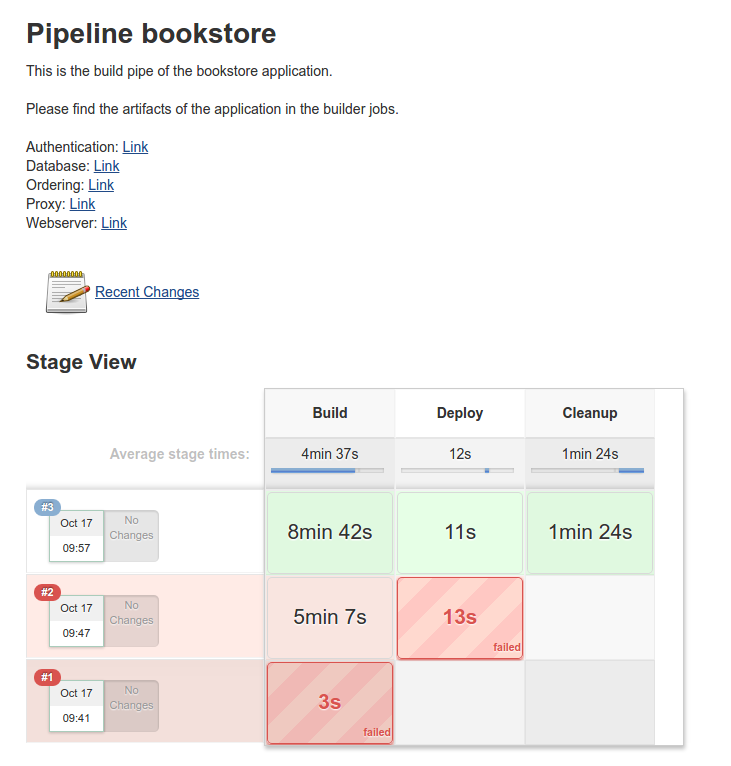
\includegraphics{img/pipeline-job.png}
\caption{Pipeline job}
\end{figure}

Amit még ajánlott alkalmazni egy ilyen rendszer kiépítése során, az egy
verzió kezelő alkalmazás, amit össze lehet kapcsolni a Jenkins-el, mivel
sok verziókezelőhöz van támogatott feladat indító feltétel (trigger).
Egy ilyen feltétel beállításai láthatók az \ref{jenkins-cred},
\ref{github-hook}, \ref{job-trigger} és \ref{job-conf} ábrákon.

Ez a változtatás lehetővé teszi, hogy a fejlesztők probléma mentesen, a
folytonos integrációt támogató eszköz ismerete nélkül is képesek
legyenek kihasználni annak előnyeit. Ehhez a funkcióhoz viszont kell
támogatás mind a Jenkins mind a GitHub oldaláról, ami azt jelenti, hogy
a GitHub-nak meg kell adni egy külső elérésű címet, amire küldheti az
adatokat, a Jenkins-nek pedig szüksége van olyan authentikációs
adatokra, amikkel csatlakozni tud a szerverhez, és változtatásokat tud
végrehajtani. Nekem sajnos nem volt külső elérésű a Jenkins szerverem,
így a triggerelést nem tudtam kipróbálni.

\begin{figure}[H]
\centering
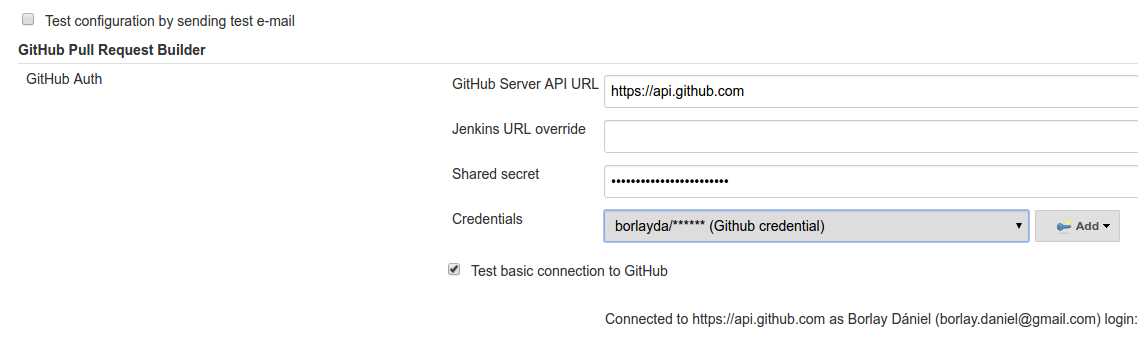
\includegraphics{img/github-cred.png}
\caption{Github beállítások a Jenkinsben\label{jenkins-cred}}
\end{figure}

Jenkins oldalról könnyen beállítható a triggerelés, mivel kapcsolódási
teszteket biztosít az eszköz, és felhasználhatóvá teszi az összes
azonosítót ami fel van véve a Jenkins-ben.

\begin{figure}[H]
\centering
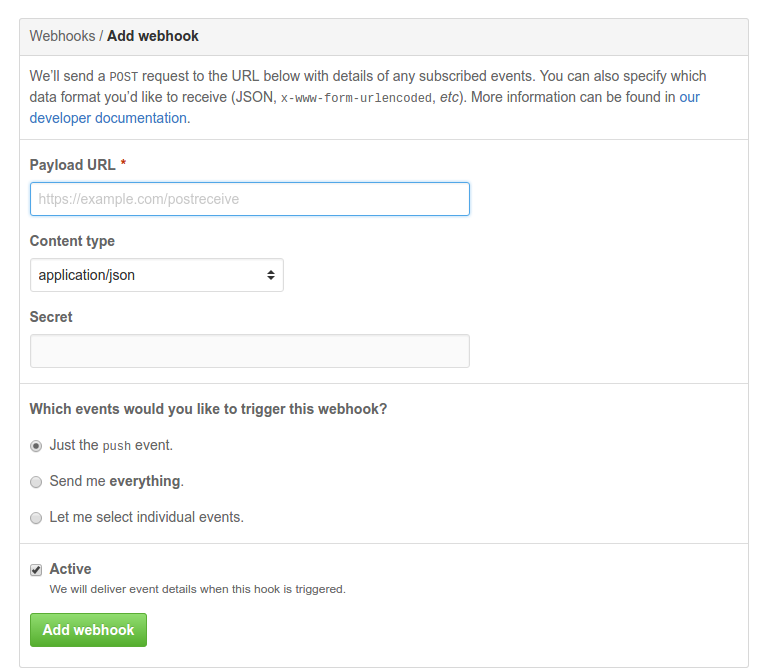
\includegraphics{img/github-webhooks.png}
\caption{Github webhook beállítás a repository
támogatásához\label{github-hook}}
\end{figure}

A GitHub oldaláról sem nehéz beállítani a kapcsolódást, viszont itt kell
megadni a publikus elérését a Jenkins szervernek, illetve egy
authentikációs kulcsot, amivel azonosítható az üzenet.

\begin{figure}[H]
\centering
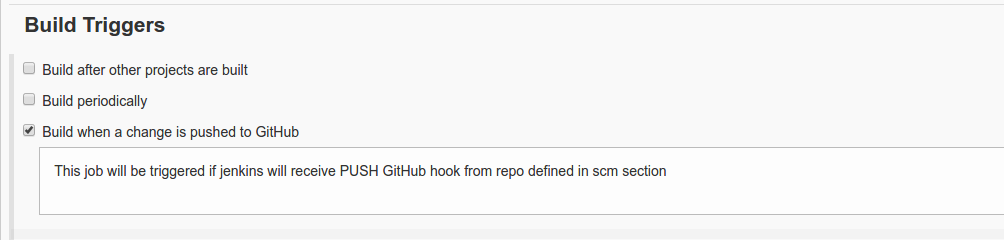
\includegraphics{img/github-trigger.png}
\caption{Github trigger beállítása egy job-on\label{job-trigger}}
\end{figure}

Az indítandó job szempontjából meg kell mondani, hogy melyik projektről
van szó, és hogy akarjuk-e, hogy változtatásokra elinduljon a job, vagy
sem.

\begin{figure}[H]
\centering
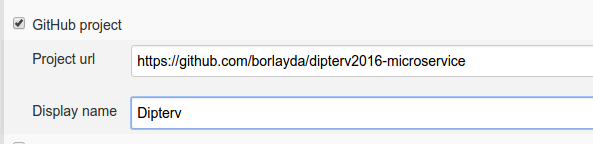
\includegraphics{img/github-job-conf.png}
\caption{Job Github-hoz rendelése\label{job-conf}}
\end{figure}

A teljesség kedvéért megemlítem, hogy nem csak a GitHub-bal lehet
összekötni a Jenkins-t ilyen céllal, hanem a Gerrit nevezetű Gites
adminisztratív eszközt, vagy más verzió kezelő eszközt melyhez találunk
telepíthető plugint.

\section{Folytonos Integrációt támogató rendszer
elkészítése}\label{folytonos-integruxe1ciuxf3t-tuxe1mogatuxf3-rendszer-elkuxe9szuxedtuxe9se}

Szerencsére könnyen és probléma mentesen tudtam dolgozni a Jenkins-el,
ami főleg annak köszönhető, hogy a szakmai gyakorlatom, és a korábbi
féléveim során is találkoztam vele. Az új funkciók nem lettek
túlbonyolítva, így könnyen tudtam kezelni a Pipeline job-ot is, csupán
rá kellett jönnöm, mely kulcsszavak mit csinálnak a konfigurációban.
Ehhez sok hasznos információt ad a Jenkins ehhez tartozó
honlapja\citep{jenkins-pipeline}. A Pipeline job-om alá szerveztem be a
buildeket, a telepítést, és a környezet kitisztítását.

A build job-ok úgy lettek meghatározva, hogy egy bash szkript hivásával
indítható legyen, és a végeredmény megjelenjen a job végeredménye
képpen. Mivel fontos lehet látni minden lépést a build folyamatában a
log-okat is csatolom a futásnál a végeredmény mellé. A telepítés
folymata is egy szkript meghívásával lett megoldva, ami Docker
konténereket indít a Jenkins-t futtató gépen. A létrehozott környezetben
lehet tesztelni bármilyen funkciót, de nekem nem volt mit tesztelnem,
így csupán a környezet indíthatósága volt a szempont. A tisztító job egy
olyan szkriptet indít el, ami törli a fájlokat a temporális
könyvtárakból, és kitisztitja a Docker-t, mint konténer, mind image
szintjén.

Minden job ugyan arra a konfigurációra épült, mivel minden job-ban volt
egyforma rész. A job-ok közös része a \ref{job-configuration} ábrán
látható.

\begin{figure}[H]
\centering
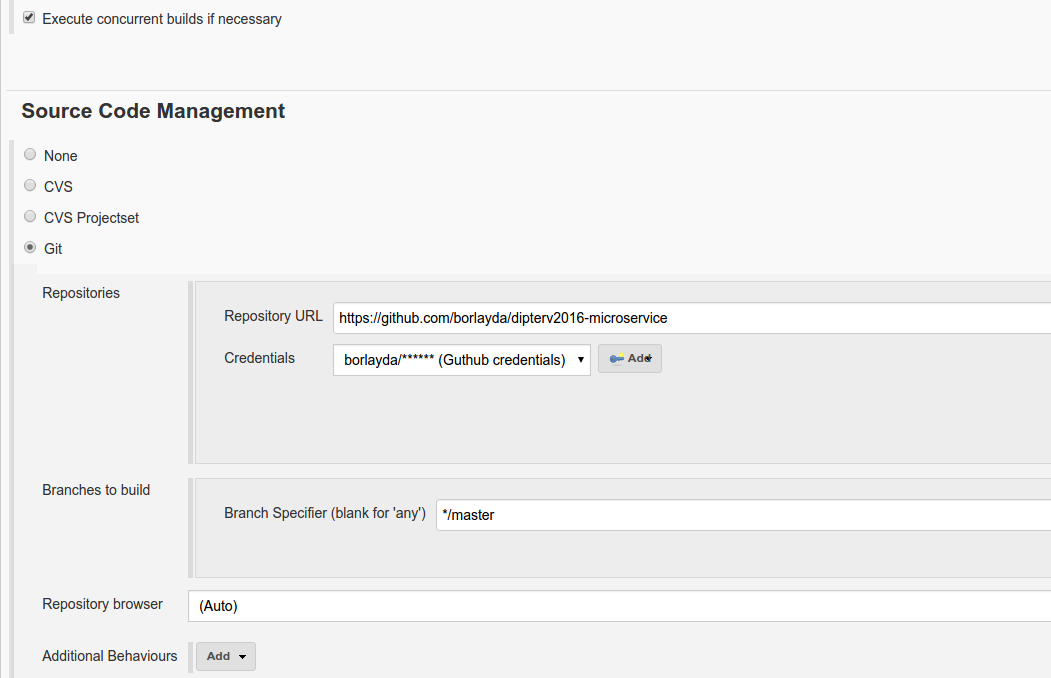
\includegraphics{img/common-job-conf}
\caption{Közös job konfiguráció\label{job-configuration}}
\end{figure}

Ami pedig különbözött minden job-ban, az a név, leírás, és a meghívott
szkript, ami a GitHub-os repository-ban található meg. Minden híváshoz a
jenkins-ben egy shell hívás tartozik, ami a következő képpen néz ki:

\begin{verbatim}
#!/bin/bash

echo "Start <Name of the phase>"
echo $PWD

./<path to script>
\end{verbatim}

Mivel minden image és build úgy lett elkészítve, hogy nyugodtan futhat
egymás mellett, a Jenkins-nek megadtam, hogy egymásra indíthatja a
feladatokat.

Ezek után kész volt a teljes folyamat, és minden használható volt. Az
egész összeállítása során, csakis a Jenkins beállításival volt gondom,
mivel a GitHub-al való összepároztatást több helyen is be kellett
állítani.

\chapter{Valós alkalmazás
értékelése}\label{valuxf3s-alkalmazuxe1s-uxe9rtuxe9keluxe9se}

Ugyan az elkészített minta alkalmazás és a folytonos integrációt
támogató keretrendszer elkészült, és működik ahogy kell, de vannak
dolgok, amiket nem teljesen úgy valósítottam meg ahogy az elmélet
elvárná, illetve vannak olyan területek ahol tovább lehetne fejleszteni
az alkalmazást.

\subsection{Tervezésbeli
eltérések}\label{tervezuxe9sbeli-eltuxe9ruxe9sek}

A Diplomaterv során megvalósított alkalmazás és folytonos integrációt
támogató keretrendszer megalkotása nem teljesen a mikroszolgáltatások
elvei szerint lettek megvalósítva, mégpedig azért, mert a tökéletes
megoldás túl sok időt emésztett volna fel, és tartalmazott volna olyan
elemeket is, amik feleslegesek lettek volna a bemutatáshoz. Az első
eltérést már leírtam, a minta alkalmazás tervezése közben, mivel az
adatbázis nem egy különálló szolgáltatás kellett volna, hogy legyen, de
nagyságrendekkel több idő lett volna megoldani, hogy minden szolgáltatás
a saját adatbázisát kezelje. Egy másik eltérés, hogy a
mikroszolgáltatásokhoz kellene tartozni egy központi kezelő felületnek,
mivel a teljes alkalmazás kezelése nehézkes, viszont a Diplomaterv
szempontjából irreleváns. Erre a célra használható egyébként a
Kubernetes nevezetű alkalmazás, ami ugyan még gyerekcipőben jár, de egy
teljes körű alkalmazás konténer kezelő rendszer, így minden kívánalmat
lefed, ami a mikroszolgáltatásokhoz kell. A Diplomaterv elkészítésénél
inkább a fejlesztési folyamat bemutatása volt a célpont, mintsem egy
kész eszköz bemutatása, így ez sem került be a félév anyagába.

\subsection{Továbbfejlesztési javaslatok, valós alkalmazásban
használandó
elemek}\label{tovuxe1bbfejlesztuxe9si-javaslatok-valuxf3s-alkalmazuxe1sban-hasznuxe1landuxf3-elemek}

Az elkészített struktúra használható ipari környezetben is, mivel a
szétválasztás adatbázisokat kezelő részét kivéve egy jó szétválasztás,
és nincs is ennél aprólékosabb, illetve a hozzá tartozó folytonos
integrációt támogató környezet is képes kezelni bármilyen komplex
alkalmazást.

Ha adott a külső elérésű Jenkins szerver, és rendelkezésre áll egy
verziókezelő program, akkor a Diplomaterv során elkészített
infrastruktúra használható a folytonos szállításhoz, és egy gyors
visszajelzést ad a fejlesztők felé, minden egyes apró változtatáshoz.
Amivel ki kell bővíteni az itt elkészült anyagot, az unit tesztek egy
halmaza a buildelendő alkalmazáshoz, funkció tesztek készítése a komplex
alkalmazás teszteléséhez, és stabilitás teszteléshez alapos stressz
teszt. Ha ezek megvannak, egy valós alkalmazás is megbízhatóan fog
működni tetszőleges környezetben.

Mivel a mikroszolgáltatások kis méretűek, és gyorsan, egyszerűen
skálázhatók, megfelelőenek tűnhet a Docker konténerek használata, de
mint már korábban mutattam, vannak limitációi, és nem túl megbízható a
használata. Ahhoz, hogy ezt kiküszöböljük erődorrásokra van szükség,
mivel kis méretű virtuális gépekben punt ugyan ilyen jól kialakítható a
rendszer, csupán meg kell oldani, hogy a Docker konténerekhez hasonló
sebességgel lehessen elindítani a szolgáltatásokat. Ezzel a
változtatással több előnyt is nyerhetünk, mivel így skálázhatók lesznek
az erőforrások a szolgáltatás alatt is és nem csak szolgáltatás
duplikációt használhatunk, illetve kiaknázva a virtualizáló eszközt amit
használunk, minotorozást, és pontos erőforrás megfigyelést is
nyerhetünk. Mivel nekem nem volt elegendő erőforrásom ennyi virtuális
gépet fenntartani, és nem volt lehetőségem valamilyen fizetős cloud
szolgáltatást felhasználva kipróbálni ezt a módszert, így ezt csak
ajánlani tudom.

Valós alkalmazás fejlesztésénél célszerűbb előre elkészíteni a folytonos
integrációt támogató keretrendszert, mivel azzal sokkal könnyebb lesz
már a kezdeti fejlesztés is, és kisebb gondot okoz a későbbi
változtatás. Amire érdemes odafigyelni, az a szolgáltatások teljesen
külön kezelése addig a pontig, amíg nem az integrált környezetet akarjuk
tesztelni, mert egy mikroszolgáltatás alapú alkalmazásnak minden kis
eleme külön termék, és így külön életciklusa van.

Ami a minta alkalmazást illeti, érdemes lehet a webes megjelenítést a
Rest-es kiszolgáló részévé tenni, mivel a Rest kommunikáció képes
kiszolgálni a böngészőből jövő HTTP kérést, de én nem ezt alkalmaztam,
mert könnyebben megvalósítható egy olyan oldal, aminek egy központi
kiszolgálója van.

\chapter{Összefoglaló}\label{uxf6sszefoglaluxf3}

A Diplomaterv során megismerkedtem a mikroszolgáltatásokra épülő
architektúrákkal illetve, hogy hogyan lehet készíteni egy alkalmazást az
elv alapján. Megismertem rengeteg olyan eszközt, amikkel meg lehet
alkotni egy jól karbantartható, skálázható, és egyszerűen formálható
rendszert, és megkerestem a legideálisabb tervezési módszereket a
metodológiával kapcsolatban. Megterveztem egy alkalmazást, ami egy
könyvesboltot valósít meg, és szétszedtem apró szolgáltatásokra, amiket
külön kezelhettem. A minta alkalmazáshoz felkonfiguráltam egy folytonos
integrációt támogató eszközt, és kipróbáltam, hogy hogyan tudja
támogatni a mikroszolgáltatásokra épülő alkalmazásomat.

A minta alkalmazás terve a praktika és a mikroszolgáltatás alapú
architektúrák elve alapján készült el, és működéséről megbizonyosodtam.
Az integrációt támogató keretrendszer a korábbi tapasztalataimra építve
készült el Jenkins folytonos integrációt támogató eszközzel, és ebben az
eszközben megvalósítottam minden szolgáltatás build-jét, a közös
integráció lépését, és egy tisztító műveletet.

A Diplomaterv eredményeként elért architektúrával tetszőleges más
mikroszolgáltatásokra épülő alkalmazásnak alapot képezhet, és apróbb
változattásokkal fel is használható.

\listoftables
\listoffigures

\bibliography{bibliography}


\appendix

\chapter{Függelék}\label{fuxfcggeluxe9k}

\section{Dockerfile-ok}\label{dockerfile-ok}

\subsection{Authentikáció}\label{authentikuxe1ciuxf3}

Dockerfile.auth.service

\begin{verbatim}
FROM ubuntu
MAINTAINER Borlay Dániel <borlay.daniel@gmail.com>

ENV CONSUL_DIR /usr/share/consul

# Install Service
COPY auth-service.py /usr/sbin/auth-service.py
RUN apt-get -y update && \
    apt-get -y install \
        vim \
        bash \
        iputils-ping \
        python-oauth \
        python-mysqldb \
        python \
        python-flask && \
    chmod +x /usr/sbin/auth-service.py

# Install consul
COPY consul consul-template /usr/bin/
RUN chmod +x /usr/bin/consul && \
    chmod +x /usr/bin/consul-template && \
    mkdir -p /etc/consul.d
COPY auth.json /etc/consul.d/auth.json

# Install entry point
COPY init /usr/sbin/init-auth
RUN chmod +x /usr/sbin/init-auth

ENTRYPOINT /bin/bash /usr/sbin/init-auth

EXPOSE 8081 8301 8302 8500 8400
\end{verbatim}

\subsection{Proxy}\label{proxy}

Dockerfile.proxy.service

\begin{verbatim}
FROM haproxy
MAINTAINER Borlay Dániel <borlay.daniel@gmail.com>

ENV CONSUL_DIR /usr/share/consul

# Install Service
COPY proxy.sh /usr/sbin/proxy.sh
RUN apt-get -y update && \
    apt-get -y --force-yes install haproxy iputils-ping && \
    chmod +x /usr/sbin/proxy.sh
COPY haproxy.cfg /etc/haproxy/haproxy.cfg

# Install consul
COPY consul consul-template /usr/bin/
RUN mkdir -p /etc/consul.d && \
    chmod +x /usr/bin/consul && \
    chmod +x /usr/bin/consul-template
COPY proxy.json /etc/consul.d/proxy.json

# Install entry point
COPY init /usr/sbin/init-proxy
RUN chmod +x /usr/sbin/init-proxy

ENTRYPOINT /bin/bash /usr/sbin/init-proxy

EXPOSE 8080 8301 8302 8500 8400
\end{verbatim}

\subsection{Adatbázis}\label{adatbuxe1zis}

Dockerfile.database.service

\begin{verbatim}
FROM ubuntu
MAINTAINER Borlay Dániel <borlay.daniel@gmail.com>

USER root
ENV CONSUL_DIR /usr/share/consul

# Install Service
COPY database.sh /usr/sbin/database.sh
COPY auth_init.sql bookstore_init.sql /tmp/
RUN apt-get -y update && \
    /bin/bash -c "debconf-set-selections <<< 'mysql-server mysql-server/root_password password root'" && \
    /bin/bash -c "debconf-set-selections <<< 'mysql-server mysql-server/root_password_again password root'" && \
    apt-get -y install mysql-server \
        iputils-ping \
        mysql-client && \
    chmod +x /usr/sbin/database.sh

# Install consul
COPY consul consul-template /usr/bin/
RUN mkdir -p /etc/consul.d && \
    chmod +x /usr/bin/consul && \
    chmod +x /usr/bin/consul-template
COPY database.json /etc/consul.d/database.json

# Install entry point
COPY init /usr/sbin/init-db
RUN chmod +x /usr/sbin/init-db && \
    sed -i 's/bind-address.*=.*/bind-address = 0.0.0.0/g' /etc/mysql/mysql.conf.d/mysqld.cnf

ENTRYPOINT /bin/bash /usr/sbin/init-db

EXPOSE 3306 8301 8302 8500 8400
\end{verbatim}

\subsection{Vásárlás}\label{vuxe1suxe1rluxe1s}

Dockerfile.order.service

\begin{verbatim}
FROM tomcat
MAINTAINER Borlay Dániel <borlay.daniel@gmail.com>

ENV CONSUL_DIR /usr/share/consul

# Install Service
RUN sed -i 's/8080/8888/g' /usr/local/tomcat/conf/server.xml && \
    sed -i 's/<Connector /<Connector address="0.0.0.0" /g' /usr/local/tomcat/conf/server.xml
COPY target/ReserveRESTJerseyExample-0.0.2-SNAPSHOT.war /usr/local/tomcat/webapps/order.war

# Install consul
COPY consul consul-template /usr/bin/
RUN mkdir -p /etc/consul.d && \
    chmod +x /usr/bin/consul && \
    chmod +x /usr/bin/consul-template
COPY order.json /etc/consul.d/order.json

# Install entry point
COPY init /usr/local/sbin/init-order
RUN chmod +x /usr/local/sbin/init-order

ENTRYPOINT /bin/bash /usr/local/sbin/init-order

EXPOSE 8888 8301 8302 8500 8400
\end{verbatim}

\subsection{Webkiszolgáló
(böngészés)}\label{webkiszolguxe1luxf3-buxf6nguxe9szuxe9s}

Dockerfile.web.service

\begin{verbatim}
FROM httpd
MAINTAINER Borlay Dániel <borlay.daniel@gmail.com>

ENV CONSUL_DIR /usr/share/consul

# Install Service
COPY webserver.sh /usr/sbin/webserver.sh
RUN apt-get -y update && \
    apt-get -y install php5 \
        php5-mysql \
        curl \
        iputils-ping \
        php5-curl && \
    chmod +x /usr/sbin/webserver.sh
COPY index.html main.css login.php store.php order.php /var/www/html/

# Install consul
COPY consul consul-template /usr/bin/
RUN mkdir -p /etc/consul.d && \
    chmod +x /usr/bin/consul && \
    chmod +x /usr/bin/consul-template
COPY web.json /etc/consul.d/web.json

# Install entry point
COPY init /usr/sbin/init-web
RUN chmod +x /usr/sbin/init-web

ENTRYPOINT /bin/bash /usr/sbin/init-web

EXPOSE 80 443 8301 8302 8500 8400
\end{verbatim}

\section{Szkriptek}\label{szkriptek}

\subsection{Futtatáshoz}\label{futtatuxe1shoz}

\subsubsection{Build}\label{build}

build\_\{service\}.sh

\begin{verbatim}
#!/bin/bash

<SERVICE>_SERVICE_HOME=services/<SERVICE>
<SERVICE>_SERVICE_DOCKERFILE=Dockerfiles/Dockerfile.<SERVICE>.service
<SERVICE>_SCRIPT_DIR=scripts/<SERVICE>
<SERVICE>_CONF_DIR=conf/<SERVICE>
<SERVICE>_IMAGE_NAME=bookstore_<SERVICE>

pushd ..
if [[ ! -e consul ]]; then
    echo "Get Consul script from Internet"
    wget https://releases.hashicorp.com/consul/0.7.0/consul_0.7.0_linux_386.zip && unzip consul_0.7.0_linux_386.zip
fi

if [[ ! -e consul-template ]]; then
    echo "Get consul-template script from Internet"
    wget https://releases.hashicorp.com/consul-template/0.16.0/consul-template_0.16.0_linux_386.zip && unzip consul-template_0.16.0_linux_386.zip
fi

echo "Create <SERVICE> service for bookstore ..."
echo " - Create directory for Docker data"
mkdir -p ${<SERVICE>_SERVICE_HOME}
echo " - Move Dockerfile to data directory"
cp ${<SERVICE>_SERVICE_DOCKERFILE} ${<SERVICE>_SERVICE_HOME}/Dockerfile
echo " - Move script files to data directory"
cp -R ${<SERVICE>_SCRIPT_DIR}/* ${<SERVICE>_SERVICE_HOME}/
echo " - Move config files to data directory"
cp -R ${<SERVICE>_CONF_DIR}/* ${<SERVICE>_SERVICE_HOME}/
echo " - Move consul to data directory"
cp consul ${<SERVICE>_SERVICE_HOME}/
cp consul-template ${<SERVICE>_SERVICE_HOME}/
echo " - Building Docker image"
docker build -t ${<SERVICE>_IMAGE_NAME} ${<SERVICE>_SERVICE_HOME} &> ${<SERVICE>_SERVICE_HOME}/build.log
echo " - Save image"
docker save --output ${<SERVICE>_SERVICE_HOME}/${<SERVICE>_IMAGE_NAME}.img ${DATABASE_IMAGE_NAME}

echo "<SERVICE> service has been created!"
popd
\end{verbatim}

\subsubsection{Futtatás}\label{futtatuxe1s}

run\_containers.sh

\begin{verbatim}
#!/bin/bash

services="database webserver order auth proxy"

docker network create bookstore

for service in ${services}
do
    echo "Start ${service} service ..."
    docker run -d --name "${service}" -h "${service}" --net=bookstore bookstore_${service}
done
\end{verbatim}

\subsubsection{Tisztogatás}\label{tisztogatuxe1s}

clean\_docker.sh

\begin{verbatim}
#!/bin/bash

services="database webserver proxy order auth"

docker stop $(docker ps -a | awk '/bookstore/ {print $1}')
docker rm $(docker ps -a | awk '/bookstore/ {print $1}')

for service in ${services}
do
    echo "Delete ${service} image"
    docker rmi bookstore_${service}
done

if [ -d services ]; then
    rm -rf services
fi
docker network rm bookstore

if [ -e consul ]; then
    rm -rf consul*
fi
\end{verbatim}

\subsection{Szolgáltatásokhoz}\label{szolguxe1ltatuxe1sokhoz}

\subsubsection{Init szkript}\label{init-szkript}

\begin{verbatim}
#!/bin/bash

IP_ADDR=$(hostname -I)
MASK=${IP_ADDR%.*}

while true; do
    FOUND=false
    for ADDR in $(seq 1 255); do
        echo "${MASK}.${ADDR}  ${IP_ADDR}"
        [[ "${MASK}.${ADDR}" == "${IP_ADDR}" ]] && continue
        ping -c 1  "${MASK}.${ADDR}"
        [ $? -eq 0 ] || continue
        echo "Try consul with ${MASK}.${ADDR}"
        consul agent -server \
                     -join "${MASK}.${ADDR}" \
                     -datacenter "bookstore" \
                     -data-dir "${CONSUL_DIR}" > /var/log/bookstore-consul.log &
        sleep 10
        cat /var/log/bookstore-consul.log
        if ps ax | grep -v grep | grep "consul" > /dev/null; then
            echo "Consul could run!!!"
            FOUND=true
            break
        fi
    done
    echo "${FOUND}"
    if [[ "${FOUND}" == "true" ]]; then
        break
    fi
done
<service>.sh
\end{verbatim}

\subsubsection{Adatbázis
inicializálás}\label{adatbuxe1zis-inicializuxe1luxe1s}

Authentikáció:

\begin{verbatim}
# Add permission to databases
GRANT ALL PRIVILEGES ON authenticate.* TO 'root'@'%';
GRANT ALL PRIVILEGES ON authenticate.* TO 'root'@'localhost';
# Create Tables
CREATE TABLE user_auth
(
    user_id int NOT NULL AUTO_INCREMENT,
    username varchar(255) NOT NULL,
    password varchar(255) NOT NULL,
    credential varchar(255),
    PRIMARY KEY (user_id)
);
# Fill Tables
INSERT INTO user_auth (username, password) VALUES ("test", "testpassword");
\end{verbatim}

Bookstore raktár:

\begin{verbatim}
# Add permission to databases
GRANT ALL PRIVILEGES ON bookstore.* TO 'root'@'%';
GRANT ALL PRIVILEGES ON bookstore.* TO 'root'@'localhost';
# Create Tables
CREATE TABLE store
(
    store_id int NOT NULL AUTO_INCREMENT,
    book_name varchar(255) NOT NULL,
    count int NOT NULL,
    PRIMARY KEY (store_id)
);
CREATE TABLE reservation
(
    reservation_id int NOT NULL AUTO_INCREMENT,
    username varchar(255) NOT NULL,
    book_name varchar(255) NOT NULL,
    count int NOT NULL,
    res_date varchar(255),
    PRIMARY KEY (reservation_id)
);
# Fill Tables
INSERT INTO store (book_name, count)
VALUES ("Harry Potter and the Goblet of fire", 10);
INSERT INTO store (book_name, count)
VALUES ("Harry Potter and the Philosopher's Stone", 10);
INSERT INTO store (book_name, count)
VALUES ("Harry Potter and the Chamber of Secret", 10);
INSERT INTO store (book_name, count)
VALUES ("Lord of the Rings: Fellowship of the ring", 3);
INSERT INTO store (book_name, count)
VALUES ("Lord of the Rings: The Two Towers", 3);
INSERT INTO store (book_name, count)
VALUES ("Lord of the Rings: The Return of the King", 0);
\end{verbatim}

\subsection{Proxy}\label{proxy-1}

Proxy config template:

\begin{verbatim}
global
    log 127.0.0.1 local1 notice
    chroot /var/lib/haproxy
    stats socket /run/haproxy/admin.sock mode 660 level admin
    stats timeout 30s
    user haproxy
    group haproxy
    daemon

defaults
    log     global
    mode    http
    option  httplog
    option  dontlognull
    timeout connect 5000
    timeout client  50000
    timeout server  50000
    errorfile 500 /etc/haproxy/errors/500.http

frontend web
    bind *:80
    mode http
    default_backend nodes

backend nodes
    mode http
    balance roundrobin{{range "app.web"}}
    service {{.ID}} {{.Address}}:{{.Port}}{{end}}

frontend database
    bind *:3306
    default_backend dbnodes

backend dbnodes
    balance roundrobin{{range "app.database"}}
    service {{.ID}} {{.Address}}:{{.Port}}{{end}}

frontend order
    bind *:8888
    default_backend onodes

backend onodes
    balance roundrobin{{range "app.order"}}
    service {{.ID}} {{.Address}}:{{.Port}}{{end}}

frontend auth
    bind *:8081
    default_backend anodes

backend anodes
    balance roundrobin{{range "app.auth"}}
    service {{.ID}} {{.Address}}:{{.Port}}{{end}}
\end{verbatim}

\end{document}
